\chapter{Distributed Delay Model}\label{section:distdel}
A systematic study of distributed delay in the context of Turing instabilities is extremely sparse in the current literature, with little to no systematic analysis of Turing pattern formation in reaction-diffusion systems with distributed delay. As far as the authors are aware, there has been no previous work carried out looking at the Schnakenberg model with incorporated distributed delay. In this chapter, we consider the LI model with time delay modelled as a (skewed) truncated Gaussian distribution. We begin this chapter by outlining the quadrature rule we use to numerically evaluate the integral term in the model \eqref{distmodel}. The linear analysis conducted for the fixed delay case is then novelly extended to the distributed delay model, and we look to show analytically, that for small mean time delay $\tau$, using either a symmetric or skewed truncated Gaussian distribution does not have a qualitative difference on the results seen, and thus does not resolve some of the key problems highlighted in the fixed delay case. These findings are verified through numerical simulations. We also conclude the same results for a larger mean time delay $\tau$ using full numerical solutions.
\section{Composite Simpson's Rule}\label{section:quad}

The LI model with distributed time delay, as defined in \eqref{distmodel}, is given by

\begin{equation}\label{distmodel2}
  \begin{split}
    \frac{\partial u}{\partial t}&=\frac{\epsilon^2}{L^2}\frac{\partial^2u}{\partial x^2}+a-u-2u^2v+3\int_{a}^{b}k(s;\textbf{p})\hat{u}^2\hat{v} \ \text{d}s,\\
    \frac{\partial v}{\partial t}&=\frac{1}{L^2}\frac{\partial^2v}{\partial x^2}+b-u^2v,
\end{split}
\end{equation}
where $\hat{u}=u(x,t-s)$ and $\hat{v}=v(x,t-s)$ and $s$ is the integration variable ranging over the delays. The integration domain $[a, b]$, can be discretised into $N$ sub-intervals of equal length with $N+1$ discretisation points, $s_0,\cdots,s_{N}$, such that $s_0=a$ and $s_N=b$. Using the composite Simpsons's rule \cite{compsimp}, the integral term can be numerically approximated as

\begin{equation}\label{simp}\int_{a}^{b}k(s)\hat{u}^2\hat{v}\  \text{d}s\approx\frac{h}{3}\left[k(s_0)\hat{u}^2_0\hat{v}_0+2\sum_{i=1}^{\frac{N}{2}-1}k(s_{2i})\hat{u}^2_{2i}\hat{v}_{2i}+4\sum_{i=2}^{\frac{N}{2}}k(s_{2i-1})\hat{u}^2_{2i-1}\hat{v}_{2i-1}+k(s_N)\hat{u}^2_N\hat{v}_N\right],
\end{equation}
where $h$ is computed as $h=\frac{b-a}{N}$. We use the notation $\hat{u}_j$ and $\hat{v}_j$ to denote $u(t-s_j)$ and $v(t-s_j$) respectively, namely the functions $u$ and $v$ evaluated at some time-delay, with index $j$, $s_j$.

\section{A Symmetric Distribution}\label{section:symmetric}
\subsection{Introduction}

As done in \cite{william}, by assuming each individual mechanism within the gene expression process acts independently and identically, we use the central limit theorem to model the delay as a symmetric Gaussian distribution with parameters $\textbf{p}=(\tau,\sigma)$, for some mean $\tau$ and standard deviation $\sigma$. Throughout Section \ref{section:symmetric}, we use integration limits $a=\tau-n\sigma$ and $b=\tau+n\sigma$ for some $n\in\mathbb{N}$, such that $a=\tau-n\sigma>0$. We can thus write the LI model with distributed time delay as

\begin{equation}\label{symmod}
    \begin{split}
        \frac{\partial u}{\partial t}&=\frac{\epsilon^2}{L^2}\frac{\partial^u}{\partial x^2}+a-u-2u^2v+3\int_{\tau-n\sigma}^{\tau+n\sigma}k(s;\tau,\sigma)\hat{u}^2\hat{v}\ \text{d}s,\\
        \frac{\partial v}{\partial t}&=\frac{1}{L^2}\frac{\partial^2v}{\partial x^2}+b-u^2.
    \end{split}
\end{equation}
The function $k(s;\tau,\sigma)$ is the symmetric truncated Gaussian pdf given by

\begin{equation}
k(s;\tau,\sigma)=\Phi_cf\left(\frac{s-\tau}{\sigma}\right).
\end{equation}
with $f(x)$ the pdf of a general (symmetric) Gaussian distribution, given as
\begin{equation}\label{f}
    f(x)=\frac{1}{\sigma\sqrt{2\pi}}\exp\left(-\frac{1}{2}x^2\right).
\end{equation}
We use $\Phi_c$ to denote the truncation scaling constant. This constant ensures that $k(s;\tau,\sigma)$ integrates to $1$ over the given integration domain $[a,b]$, and is computed as
\begin{equation}
    \Phi_c=\frac{1}{\phi\left(\frac{b-\tau}{\sigma}\right)-\phi\left(\frac{a-\tau}{\sigma}\right)},
\end{equation}
with $\phi(x)$ the cdf of the (symmetric) standard Gaussian distribution. This is given by
\begin{equation}\label{phi}
    \phi(x)=\frac{1}{2}\left(1+\text{erf}\left(\frac{x}{\sqrt{2}}\right)\right).
\end{equation}

Throughout this section we use $n=3$ so that the integration limits are $a=\tau-3\sigma$ and $b=\tau+3\sigma$. This was chosen so that a relatively large $\sigma$ value could be chosen for each $\tau$ while maintaining $a>0$. For each $\tau$ value, a maximum $\sigma$ value can be computed such that $a=\tau-3\sigma\geq0$ as $\sigma_{\max}=\frac{\tau}{3}$. By setting $\sigma<\sigma_{\max}$, we ensure that the integration domain strictly considers positive time delays only.

Figures \ref{fig:pdf1} and \ref{fig:pdf2} show the pdf of a truncated Gaussian distribution centred at a mean $\tau=1,2$ with varying $\sigma$ values as fractions of $\sigma_{max}$.

\begin{figure}[H]
    \centering
    \begin{subfigure}[t]{0.45\textwidth}
        \centering
        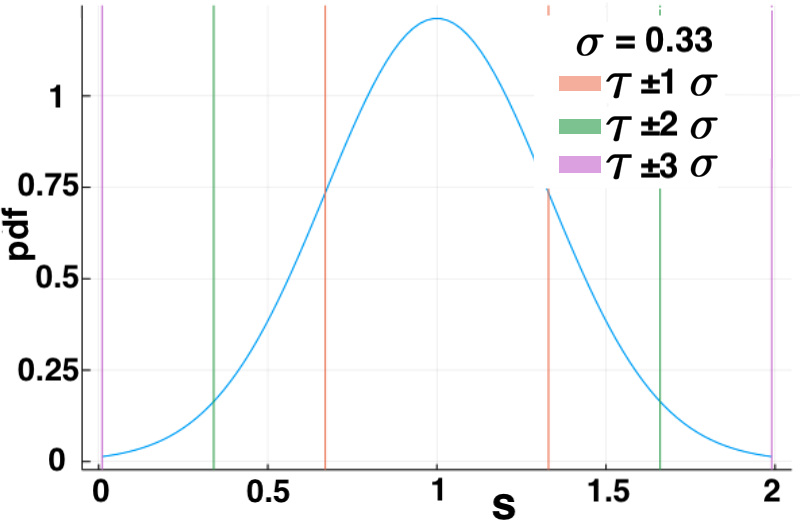
\includegraphics[width=7cm,height=4.5cm]{t1sig1.png}
        \caption{Truncated Gaussian distribution following $\mathcal{N}(1,(\sigma_{max}\times0.99)^2)$}
        \label{}
    \end{subfigure}
    \hfill
    \begin{subfigure}[t]{0.45\textwidth}
        \centering
        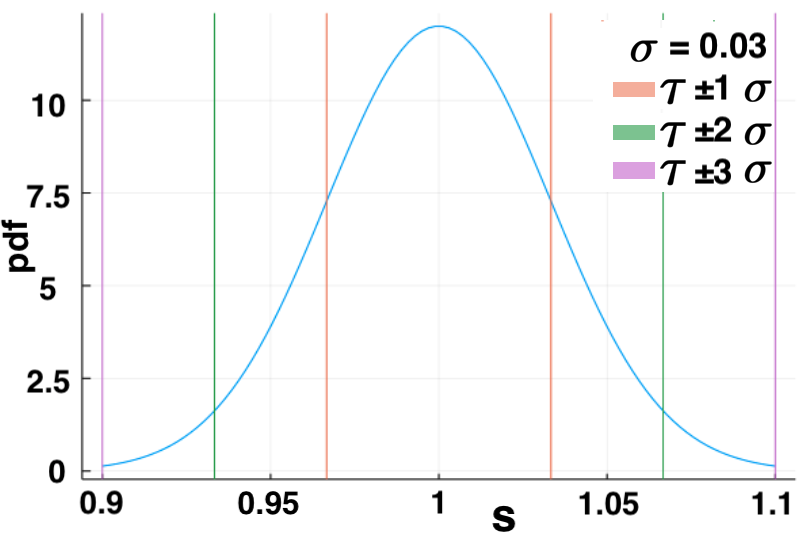
\includegraphics[width=7cm,height=4.5cm]{t1sig2.png}
        \caption{Truncated Gaussian distribution following $\mathcal{N}(1,(\sigma_{max}\times0.1)^2)$}
        \label{}
    \end{subfigure}
\caption{PDF of truncated symmetric Gaussian distribution with mean $\tau=1$ and integration domain $[1-3\sigma,1+3\sigma]$. $\sigma$ values of $0.33(2.d.p)$ and $0.03(2.d.p)$ are considered.}
\label{fig:pdf1}
\end{figure}
\begin{figure}[H]
    \centering
    \begin{subfigure}[t]{0.45\textwidth}
        \centering
        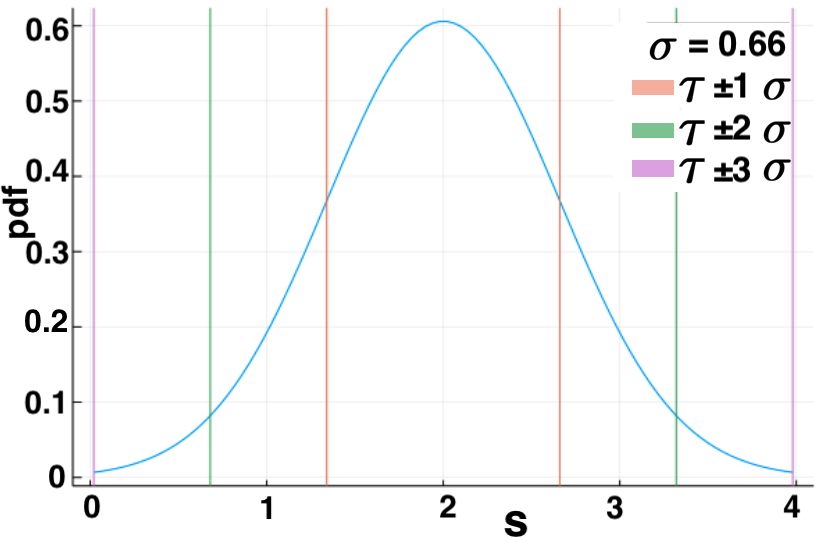
\includegraphics[width=7cm,height=4.5cm]{t2sig1.png}
        \caption{Truncated Gaussian distribution following $\mathcal{N}(2,(\sigma_{max}\times0.99)^2)$}
        \label{}
    \end{subfigure}
    \hfill
    \begin{subfigure}[t]{0.45\textwidth}
        \centering
        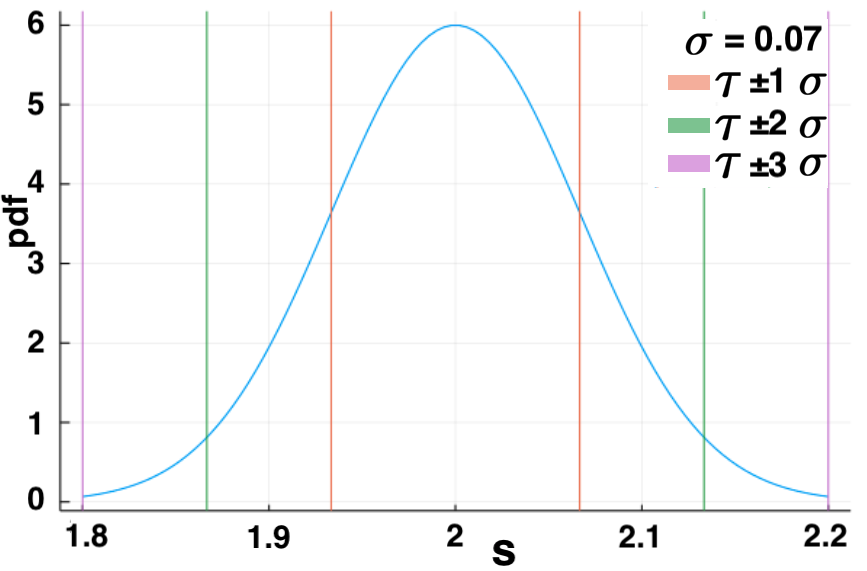
\includegraphics[width=7cm,height=4.5cm]{t2sig2.png}
        \caption{Truncated Gaussian distribution following $\mathcal{N}(2,(\sigma_{max}\times0.1)^2)$}
        \label{}
    \end{subfigure}
    \caption{PDF of symmetric truncated Gaussian distribution with mean $\tau=2$ and integration domain $[2-3\sigma,2+3\sigma]$. $\sigma$ values of $0.66(2.d.p)$ and $0.07(2.d.p)$ are considered.}
    \label{fig:pdf2}
\end{figure}
We see that $\sigma$ is responsible for scaling on the $x$-axis, while the truncation constant $\Phi_c$, defined in \eqref{distmodel}, scales the $y$-axis, ensuring the pdf integrates to $1$ across the integration domain. Throughout Chapter \ref{section:distdel}, the number of sub-intervals $N$ was chosen to be $N=50$ for the implementation of the quadrature rule applied to the distribution of delay (for both symmetric and skewed distributions). The consideration for such a choice involves both quadrature accuracy and computational efficiency. In this section, we present results obtained in testing the quadrature rule, to show that $N=50$ is a sufficiently large choice. We apply the quadrature to two test integrals: the first is the truncated Gaussian pdf $k(s;\tau,\sigma)$, which should analytically integrate to $1$. For the second test, we apply the quadrature rule to both a spatially and temporally dependent integral
\begin{equation}\label{testint}
\int_a^bk(s;\tau,\sigma)f(x,t-s)\ \text{d}s,
\end{equation}
where $f(x,t)=xt$. This can be explicitly evaluated as

\begin{equation}
    \begin{split}
&\int_a^bk(s;\tau,\sigma)f(x,t-s)\ \text{d}s=xt\int_a^bk(s;\tau,\sigma)\ \text{d}s-x\int_a^bk(s;\tau,\sigma)s\ \text{d}s\\&=xt\left[\frac{\Phi_c}{2}\text{erf}\left(\frac{s-\tau}{\sqrt{2}\sigma}\right)\right]\bigg|_a^b-x\left[\frac{\Phi_c}{2}\text{erf}\left(\frac{s-\tau}{\sqrt{2}\sigma}\right)-\frac{\Phi_c\sigma}{\sqrt{2\pi}}\exp\left(-\frac{1}{2}\left(\frac{s-\tau}{\sigma}\right)^2 \right)\right]\Bigg|_a^b.
    \end{split}
\end{equation}

Figures in appendix \ref{section:appB} show the relative (and absolute error) of the quadrature rule applied to the truncated Gaussian pdf $k(s;\tau,\sigma)$ for different $N$, with varying $\tau$ and $\sigma$. Figures also show the relative error of the quadrature rule applied to \eqref{testint} for $t\in[1.1,500]$ and $x\in[0.1,1]$, for a varying $\tau$ and $\sigma$, with $N=50$. The spatial and temporal domains were chosen to discard the effects of catastrophic cancellation, which is caused by very small solution values for $0\leq t\leq 1.1$ and $0\leq x\leq 0.1$. The results show that the relative error (in absolute value) of the composite Simpson's rule applied to both test integrals, with $N=50$, is of $O(10^{-4})$, namely $<0.1\%$ error, independent of $\tau$ and $\sigma$, across both spatial and temporal domains. We therefore conclude that using $N=50$ quadrature points is sufficiently large.


\subsection{Linear Analysis}\label{section:distlin}
Taking a small perturbation about the steady-state $u=u_\star+\delta\xi$, $v=v_\star+\delta\eta$, where $|\delta|\ll1$, we can write the equation for the activator $u$ in \eqref{distmodel2} as

\begin{equation}\label{perturb}
  \delta\frac{\partial \xi}{\partial t}=\delta \frac{\epsilon^2}{L^2}\frac{\partial^2\xi}{\partial x^2}+f(u_\star+\delta\xi, v_\star+\delta\eta)+g(u_\star+\delta\hat{\xi},v_\star+\delta\hat{\eta}) ,
\end{equation}
where $f(u,v)=a-u+2u^2v$ and $g(\hat{u},\hat{v})=3\int_a^bk(s)\hat{u}^2\hat{v}\ \text{d}s$. The $\hat{\xi}$ notation is used to denote the perturbation evaluated at a delay $\hat{\xi}=\xi(x,t-s)$. Taylor expanding equation \eqref{perturb} for the $f$ term about the steady-state and evaluating the $g$ term, up to $O(\delta)$, yields

\begin{dmath}\label{taylor}
  \delta\frac{\partial \xi}{\partial t}=\delta \frac{\epsilon^2}{L^2}\frac{\partial^2\xi}{\partial x^2}+f(u_\star,v_\star)+3u_\star^2v_\star\int_a^bk(s)\ \text{d}s+\delta\left[\xi f_u(u_\star,v_\star)+\eta f_v(u_\star,v_\star)+6u_\star v_\star\int_a^bk(s)\hat{\xi}\text{d}s+3u_\star^2\int_a^bk(s)\hat{\eta}\ \text{d}s
  \right].
\end{dmath}
We use the notation $f_u$ to denote the derivative of function $f$ with respect $u$. Using the fact that the pdf $k(s;\tau,\sigma)$ integrates to $1$ over $[a,b]$, and evaluating the expressions $f_u(u_\star,v_\star)$ and $f_v(u_\star,v_\star)$, equation \eqref{taylor} can be simplified to

\begin{equation}\label{linu}
  \delta \frac{\partial \xi}{\partial t}=\delta \frac{\epsilon^2}{L^2}\frac{\partial^2\xi}{\partial x^2}+\delta\left[\xi(-1-4u_\star v_\star)-2\eta u_\star^2 +6u_\star v_\star\int_a^bk(s)\hat{\xi}\ \text{d}s+3u_\star^2\int_a^bk(s)\hat{\eta}\ \text{d}s\right].
\end{equation}
The linearised dynamics for $v$ are more simply given by
\begin{equation}\label{linv}
\delta \frac{\partial\eta}{\partial t}=\delta \frac{1}{L^2}\frac{\partial^2\eta}{\partial x^2}-\delta\left[2\xi u_\star v_\star+\eta u_\star^2\right].
\end{equation}
Dividing through by $\delta$ and substituting in an ansatz of the form $\xi=\xi_0e^{\lambda_k t}\cos(k\pi x)$ \cite{yigaffneyli} into \eqref{linu} and $\eta=\eta_0e^{\lambda_k t}\cos(k\pi x)$ into \eqref{linv}, and then dividing through by $e^{\lambda_k t}\cos(k\pi x)$, results in
\begin{equation}\label{sysof}
  \begin{split}
\lambda_k\xi_0&=-\frac{\epsilon^2}{L^2}k^2\pi^2\xi_0+\xi_0(-1-4u_\star v_\star)-2\eta_0u_\star^2+6\xi_0u_\star v_\star E_k+3\xi_0u_\star^2E_k \\
\lambda_k\eta_0&=-\frac{1}{L^2}k^2\pi^2\eta_0-2\xi_0u_\star v_\star-\eta_0u_\star^2,
\end{split}
\end{equation}
where $E_k=\int_a^bk(s;\tau,\sigma)e^{-\lambda_k s}\ \text{d}s$. We can write equation \eqref{sysof} as a homogeneous linear system for $(\xi_0,\eta_0)^T$, given by

\begin{equation}
\underbrace{\begin{pmatrix}-1-4u_\star v_\star-\frac{\epsilon^2}{L^2}k^2\pi^2+6u_\star v_\star E_k-\lambda_k&-2u_\star^2+3u_\star^2E_k\\-2u_\star v_\star&-u_\star^2-\frac{1}{L^2}k^2\pi^2-\lambda_k \end{pmatrix}}_{\textbf{M}}\begin{pmatrix}\xi_0\\\eta_0\end{pmatrix}=\begin{pmatrix}0\\0\end{pmatrix}.
\end{equation}
Looking for non-trivial solutions, we look for roots of the characteristic equation, namely $\mathcal{D}_k=\text{det}(\textbf{M})=0$. The characteristic equation is given as
\begin{equation}\label{characdist}
  \mathcal{D}_k=\lambda_k^2+\alpha_k\lambda_k+\beta_k+(\gamma_k\lambda_k+\delta_k)E_k=0,
\end{equation}
where
\begin{equation}\label{characcoeff}
    \begin{split}
\alpha_k&=\left(\frac{\epsilon^2}{L^2}+\frac{1}{L^2}\right)k^2\pi^2+u_\star^2+4u_\star v_\star+1,\\
\beta_k&=\left(\frac{1}{L^2}\pi^2k^2+u_\star^2\right)\left(\frac{\epsilon^2}{L^2}\pi^2k^2+4u_\star v_\star+1\right)-4u_\star^3v_\star,\\
\gamma_k&=-6u_\star v_\star,\\
\delta_k&=-\frac{6}{L^2}u_\star v_\star k^2\pi^2.
\end{split}
\end{equation}

Finally, we note that the expression $E_k$ can be evaluated explicitly as
\begin{equation}
E_k=\int_a^bk(s;\tau,\sigma)e^{-\lambda_k s}\ \text{d}s=\frac{\Phi_c}{2}\left[\exp\left(\frac{\lambda_k(\lambda_k\sigma^2-2\tau)}{2}\right) \text{erf} \left(\frac{\lambda_k\sigma^2+s-\tau}{\sqrt{2}\sigma}\right)\right]\Bigg|_a^b.
\end{equation}
The charactersitic equation \eqref{characdist} cannot trivially be split into its real and imaginary components, due to the error function term in $E_k$, as was done in the fixed delay case. We therefore cannot explicitly compute the stability lines in $(a,b)$ parameter space. We can however range over $(a,b)$ and compute $\max_k(\Re(\lambda_k))$ for different $\tau$, and produce plots similar to those in figures \ref{fig:dispfixed} and \ref{fig:lambdavary}. We use these plots to pseudo-analytically prove that, using a symmetric Gaussian distribution centred at mean $\tau$ will not change the time-to-pattern seen for a fixed delay of $\tau$, independent of the standard deviation of the distribution $\sigma$. We first plot $\max_k(\Re(\lambda_k))$ against $\tau$, as seen analogously in figure \ref{fig:dispfixed} for the fixed delay case, for multiple parameters $(a,b,\tau,\sigma)$, and compares these to the fixed delay case.

Figures \ref{fig:p2} and \ref{fig:p3} show $\max_k(\Re(\lambda_k))$ plotted against $\tau\in[0,1]$ for two different parameter sets $(a,b)=\{(0.1,0.9), (0.4,0.4)\}$, for the fixed delay case. For each parameter set, figures are produced with different $\sigma$ values as a fraction of $\sigma_{max}$, and the absolute value of the difference between $\max_k(\Re(\lambda_k))$ for each distributed delay case compared with the fixed delay case is plotted. We note that in the distributed delay case,  $\sigma_{max}$ and thus the integration limits both change as functions of $\tau$. All numerical results in this chapter are produced with $L^2=9/2$, and unless otherwise stated, $\epsilon^2=0.001$.

% PARAMTER SET 2
\begin{figure}[H]
    \centering
    \begin{subfigure}[t]{0.45\textwidth}
        \centering
        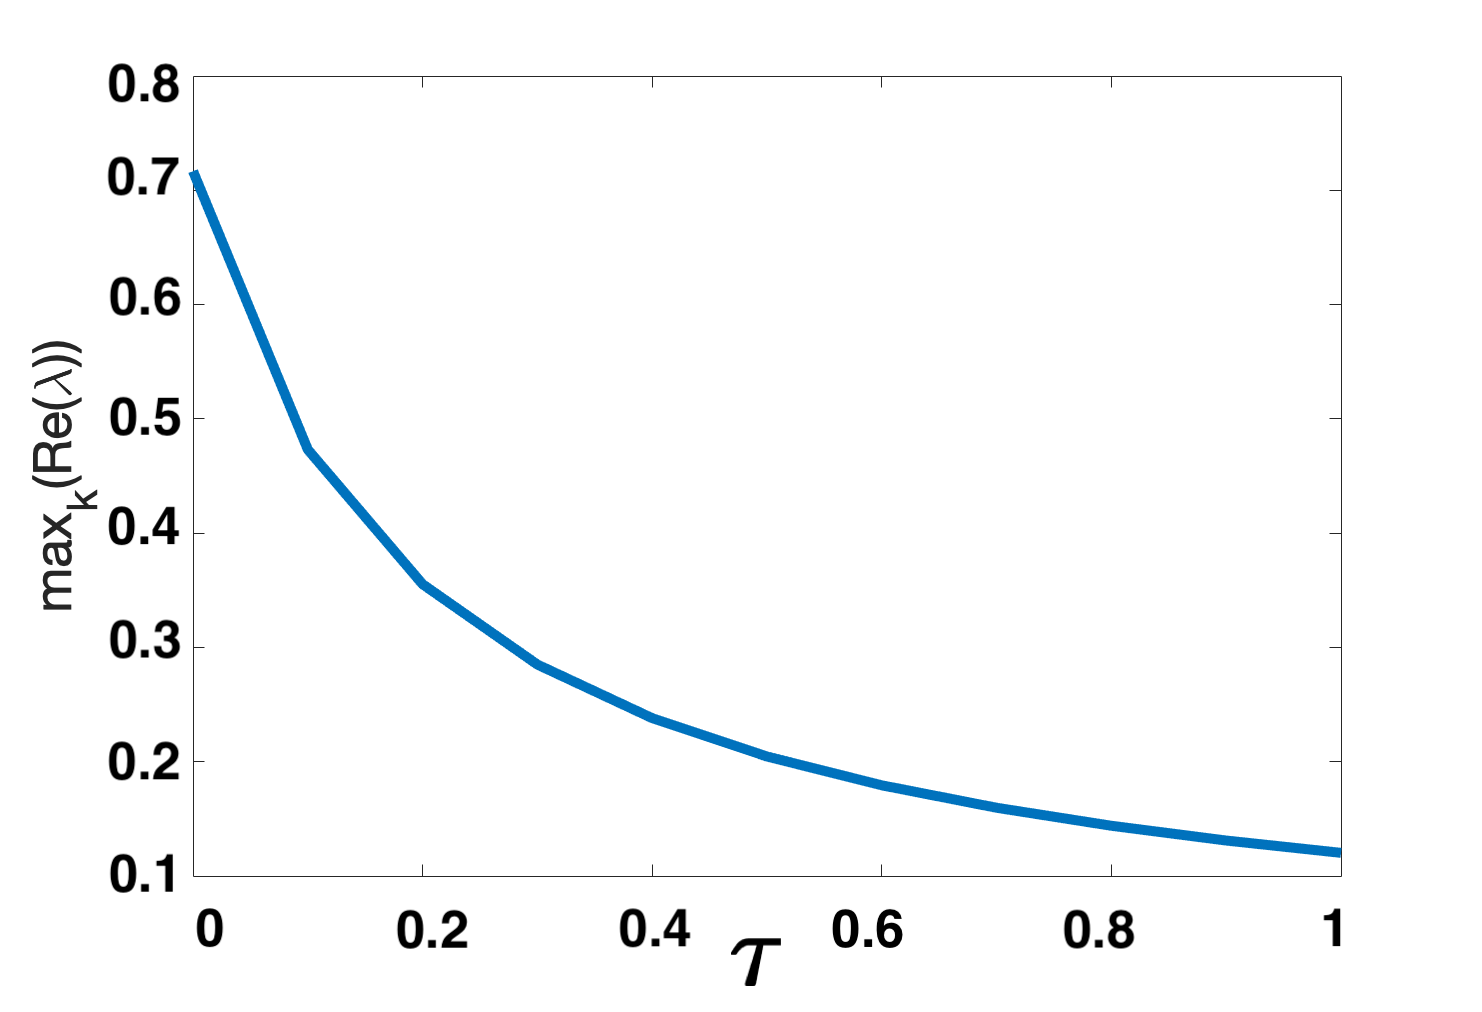
\includegraphics[width=7cm,height=5cm]{p2fixed.png}
        \caption{$\max_k(\Re(\lambda_k))$ plotted for fixed delay case.}
        \label{}
    \end{subfigure}
    \hfill
    \begin{subfigure}[t]{0.45\textwidth}
        \centering
        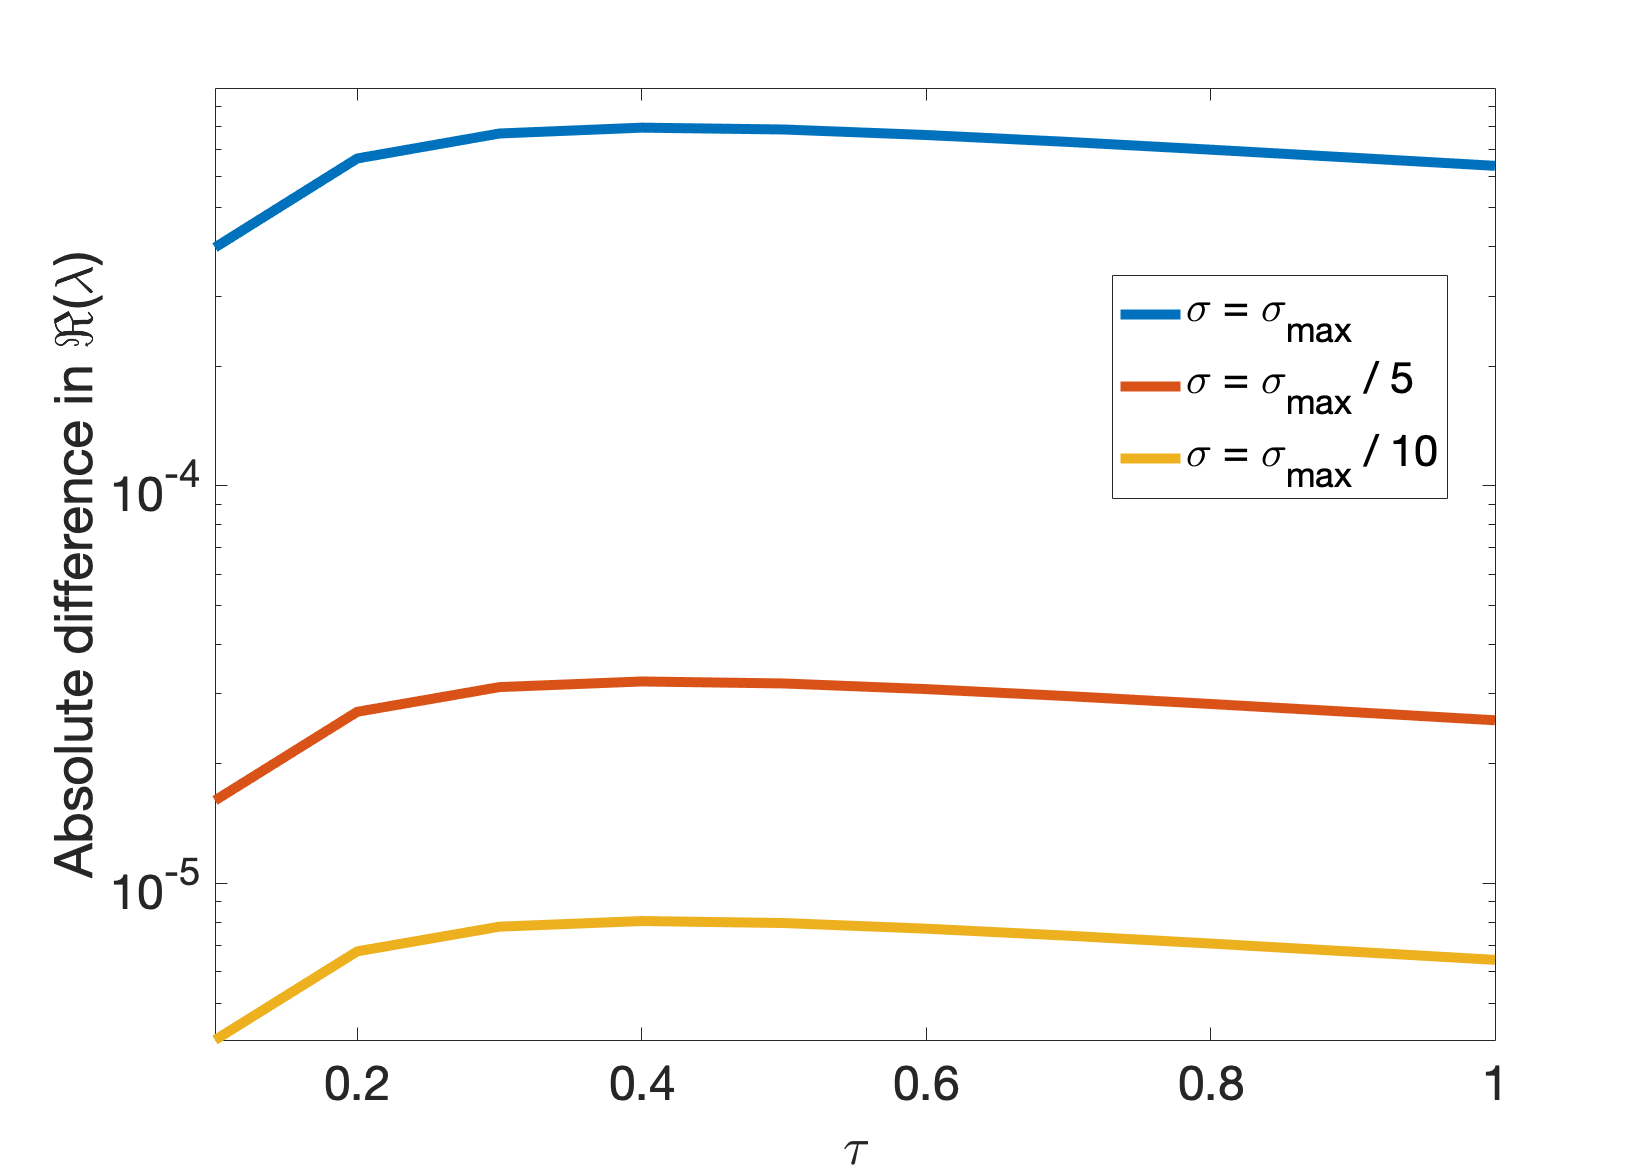
\includegraphics[width=7cm,height=5cm]{dispdiff1.png}
        \caption{Absolute difference in $\max_k(\Re(\lambda_k))$ as $\sigma$ is varied, between each distributed delay case and the fixed delay case.}
        \label{}
    \end{subfigure}
    \caption{$\max_k(\Re(\lambda_k))$ plotted against $\tau\in[0,1]$ for parameter set $(a,b)=(0.1,0.9)$. $\epsilon^2=0.001$ and $L^2=9/2$. $k\in\mathbb{Z}$ is varied over $[0,50]$. Absolute difference of $\max_k(\Re(\lambda_k))$ between each of the distributed delay cases and fixed delay case plotted.}
    \label{fig:p2}
\end{figure}
% PARAMETER SET 3
\begin{figure}[H]
    \centering
    \begin{subfigure}[t]{0.45\textwidth}
        \centering
        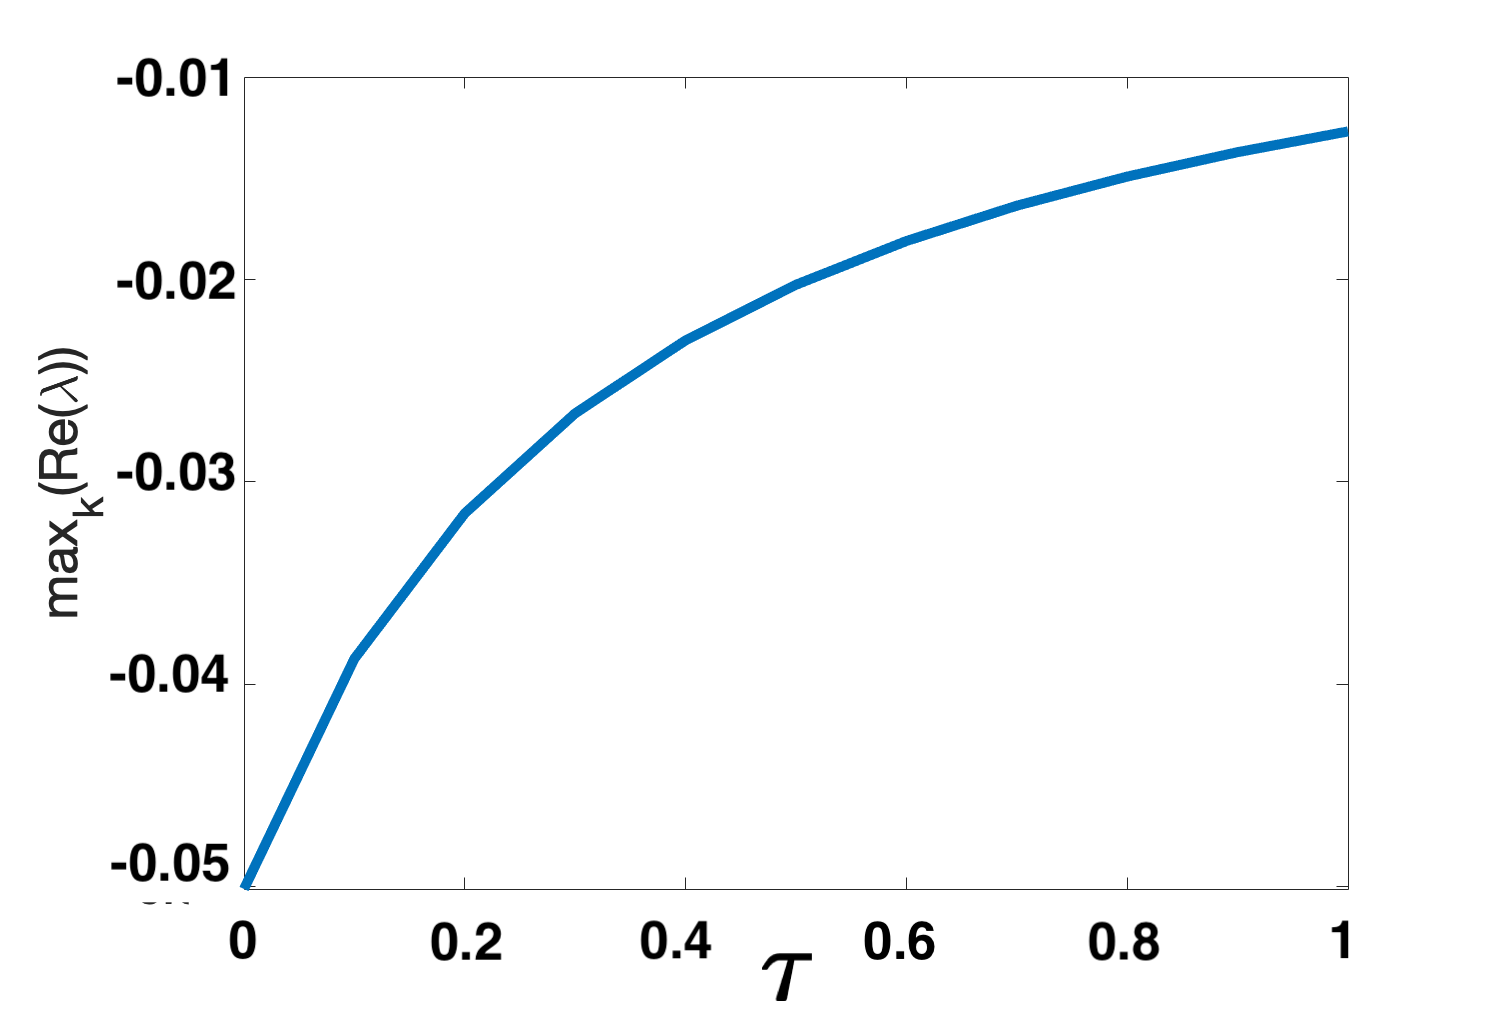
\includegraphics[width=7cm,height=5cm]{p3fixed.png}
        \caption{$\max_k(\Re(\lambda_k))$ plotted for fixed delay case.}
        \label{}
    \end{subfigure}
    \hfill
    \begin{subfigure}[t]{0.45\textwidth}
        \centering
        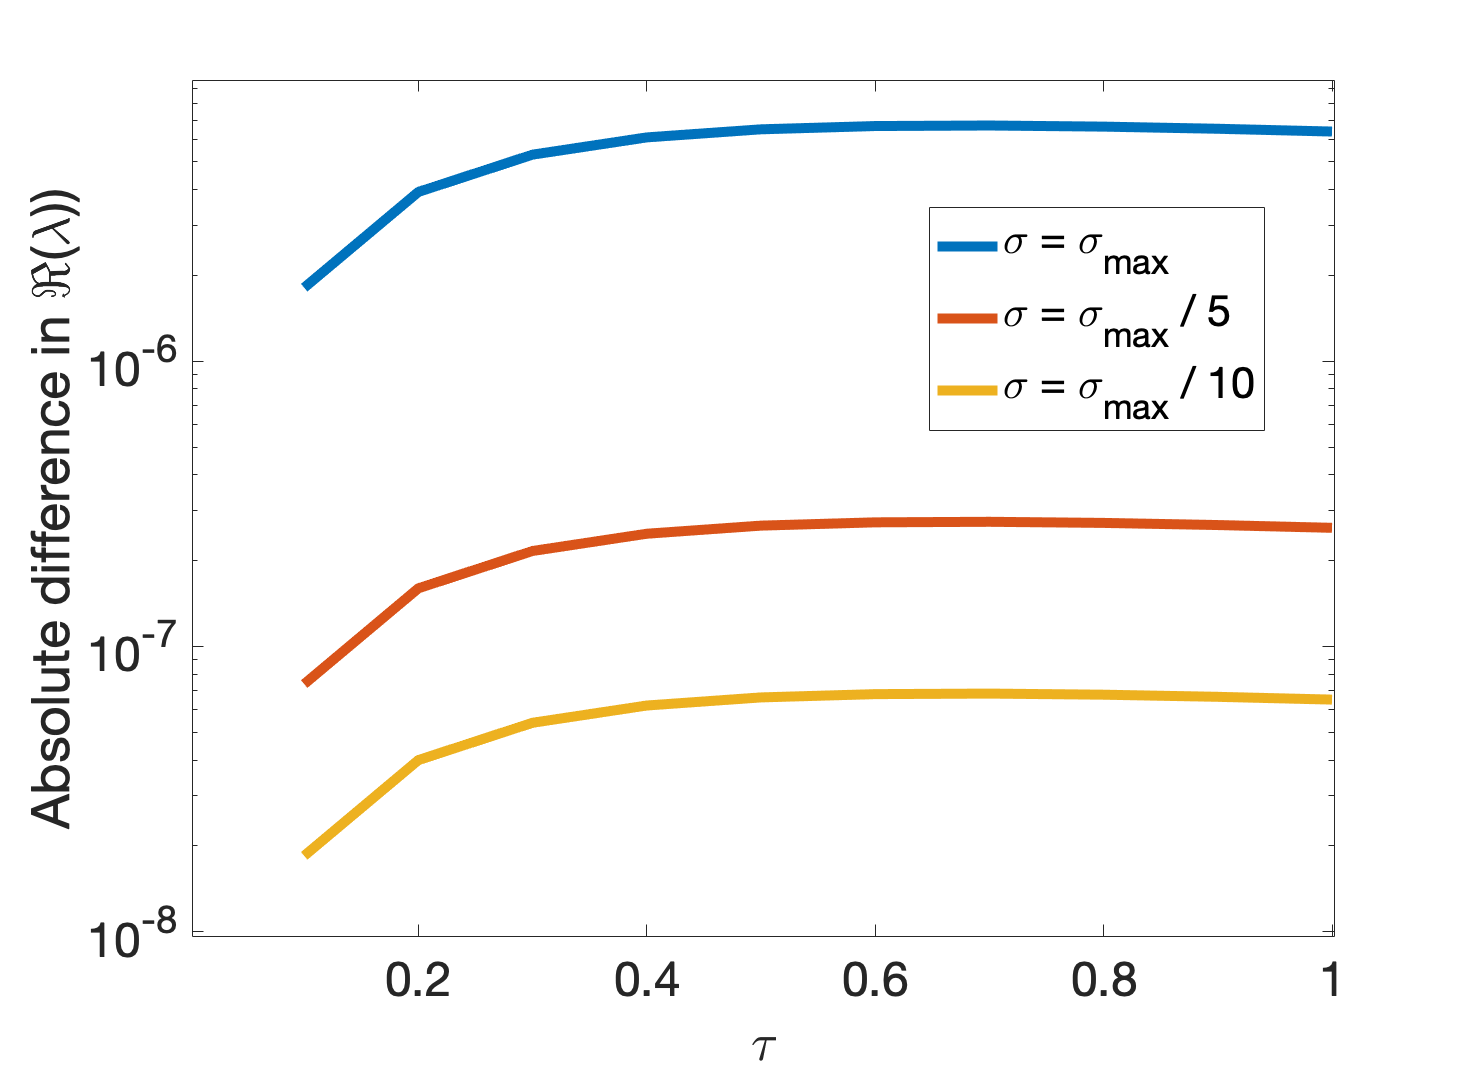
\includegraphics[width=7cm,height=5cm]{dispdiff2.png}
        \caption{Absolute difference in $\max_k(\Re(\lambda_k))$ as $\sigma$ is varied, between each distributed delay case and the fixed delay case.}
        \label{}
    \end{subfigure}
    \caption{$\max_k(\Re(\lambda_k))$ plotted against $\tau\in[0,1]$ for parameter set $(a,b)=(0.4,0.4)$. $\epsilon^2=0.001$ and $L^2=9/2$. $k\in\mathbb{Z}$ is varied over $[0,50]$. Absolute difference of $\max_k(\Re(\lambda_k))$ between each of the distributed delay cases and fixed delay case plotted.}
    \label{fig:p3}
\end{figure}

Figures \ref{fig:p2} and \ref{fig:p3} show that, the largest difference in $\max_k(\Re(\lambda_k))$ when the largest $\sigma$ value is used. The results also suggest that for all $\sigma$ and $\tau\in[0,1]$ considered, that we expect to see pattern formation for $(a,b)=(0.1,0.9)$, but not for $(a,b)=(0.4,0.4)$. We note that that largest absolute difference in $\max_k(\Re(\lambda_k))$ across both parameter sets is of $O(10^{-3})$. This is an extremely small difference and is thus unlikely to make a qualitative difference on the rate of growth of a perturbation, and thus time-to-pattern. We verify these obvservations numerically in section \ref{section:distsim}.

In order to consider how $\max_k(\Re(\lambda_k))$ varies across a larger parameter plane as $\sigma$ is varied, we consider the absolute difference of $\max_k(\Re(\lambda_k))$ for varying $\sigma$ values as a fraction of $\sigma_{max}$, for multiple $\tau$, against the fixed delay case, for $\epsilon^2=0.001,0.01$. For each $(\tau,\epsilon^2)$, bifurcation plots were computed for the distributed delay case with varying $\sigma\in\{\sigma_{\max}\times0.99,\sigma_{\max}\times0.2,\sigma_{\max}\times0.1\}$. For each $(\tau,\epsilon^2)$, we consider the absolute difference of $\max_k(\Re(\lambda_k))$ between each distributed delay case and the fixed delay case, across the $(a,b)$ parameter space. These results are summarised in table \ref{tab:tab1}. The bifurcation diagrams of $\max_k(\Re(\lambda_k))$ across the $(a,b)$ space can be found in Appendix \ref{section:appB}
% \begin{figure}[H]
%     \centering
%     \begin{subfigure}[t]{0.45\textwidth}
%         \centering
%         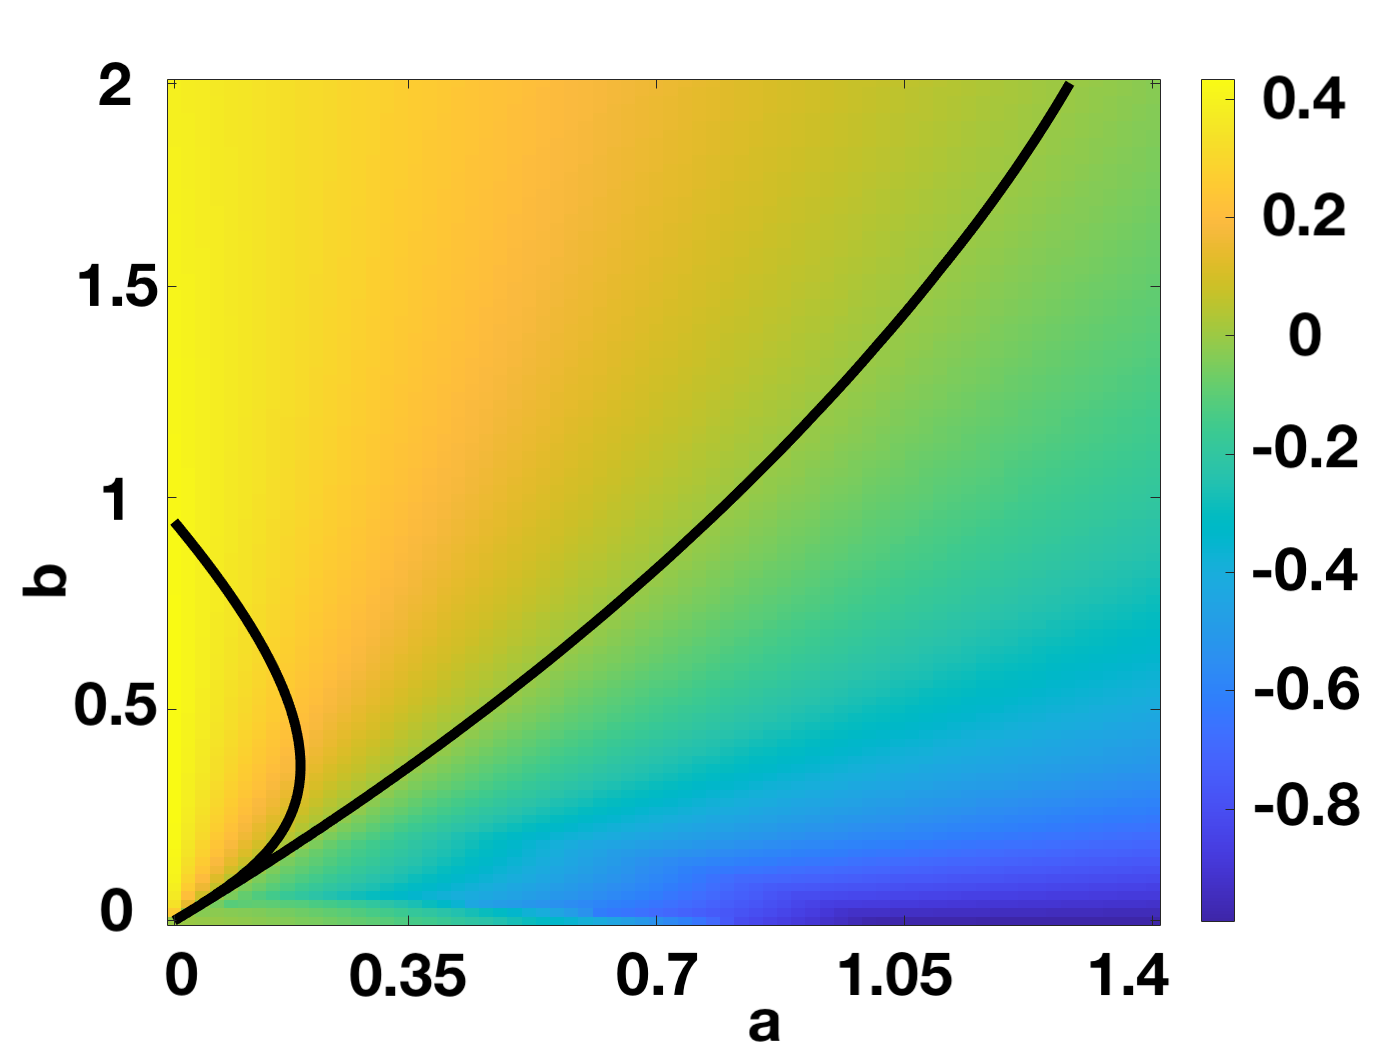
\includegraphics[width=7cm,height=4.75cm]{t1f1.png}
%         \caption{$\tau=0.2$.}
%         \label{}
%     \end{subfigure}
%     \hfill
%     \begin{subfigure}[t]{0.45\textwidth}
%         \centering
%         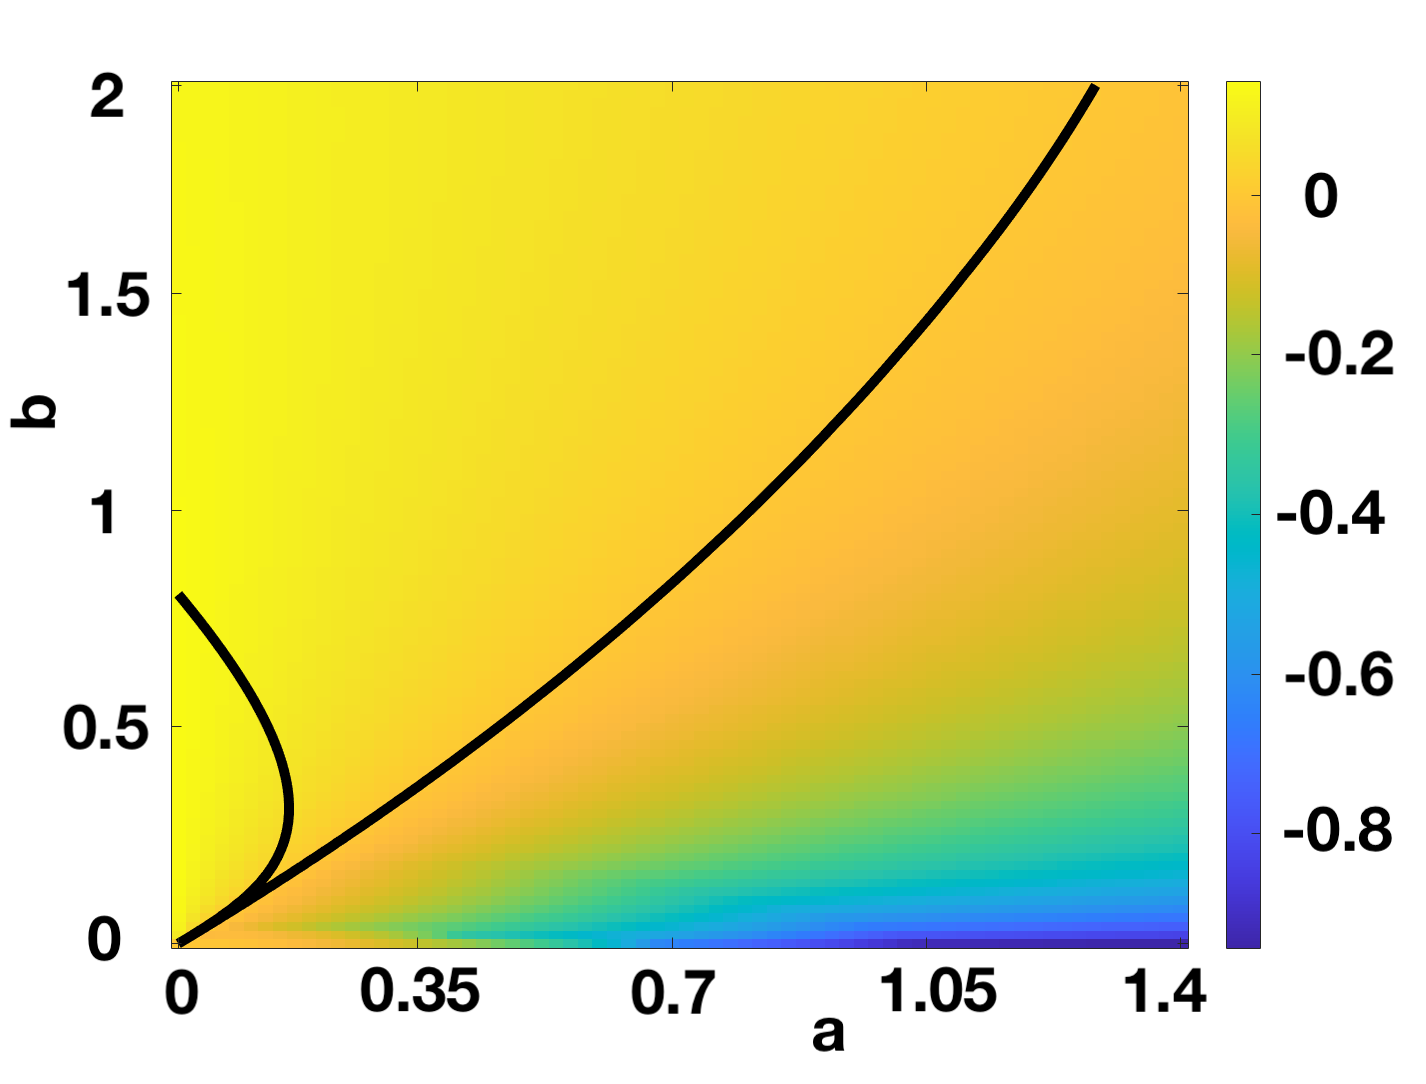
\includegraphics[width=7cm,height=4.75cm]{t2f1.png}
%         \caption{$\tau=1$}
%         \label{}
%     \end{subfigure}
%     \caption{Bifurcation diagrams produced by solving \eqref{characfix} (fixed delay characteristic equation) for $\tau=0.2,1$ and $\epsilon^2=0.001$, on a domain length $L^2=9/2$.}
%     \label{fig:distheat1}
% \end{figure}
% \begin{figure}[H]
%     \centering
%     \begin{subfigure}[t]{0.45\textwidth}
%         \centering
%         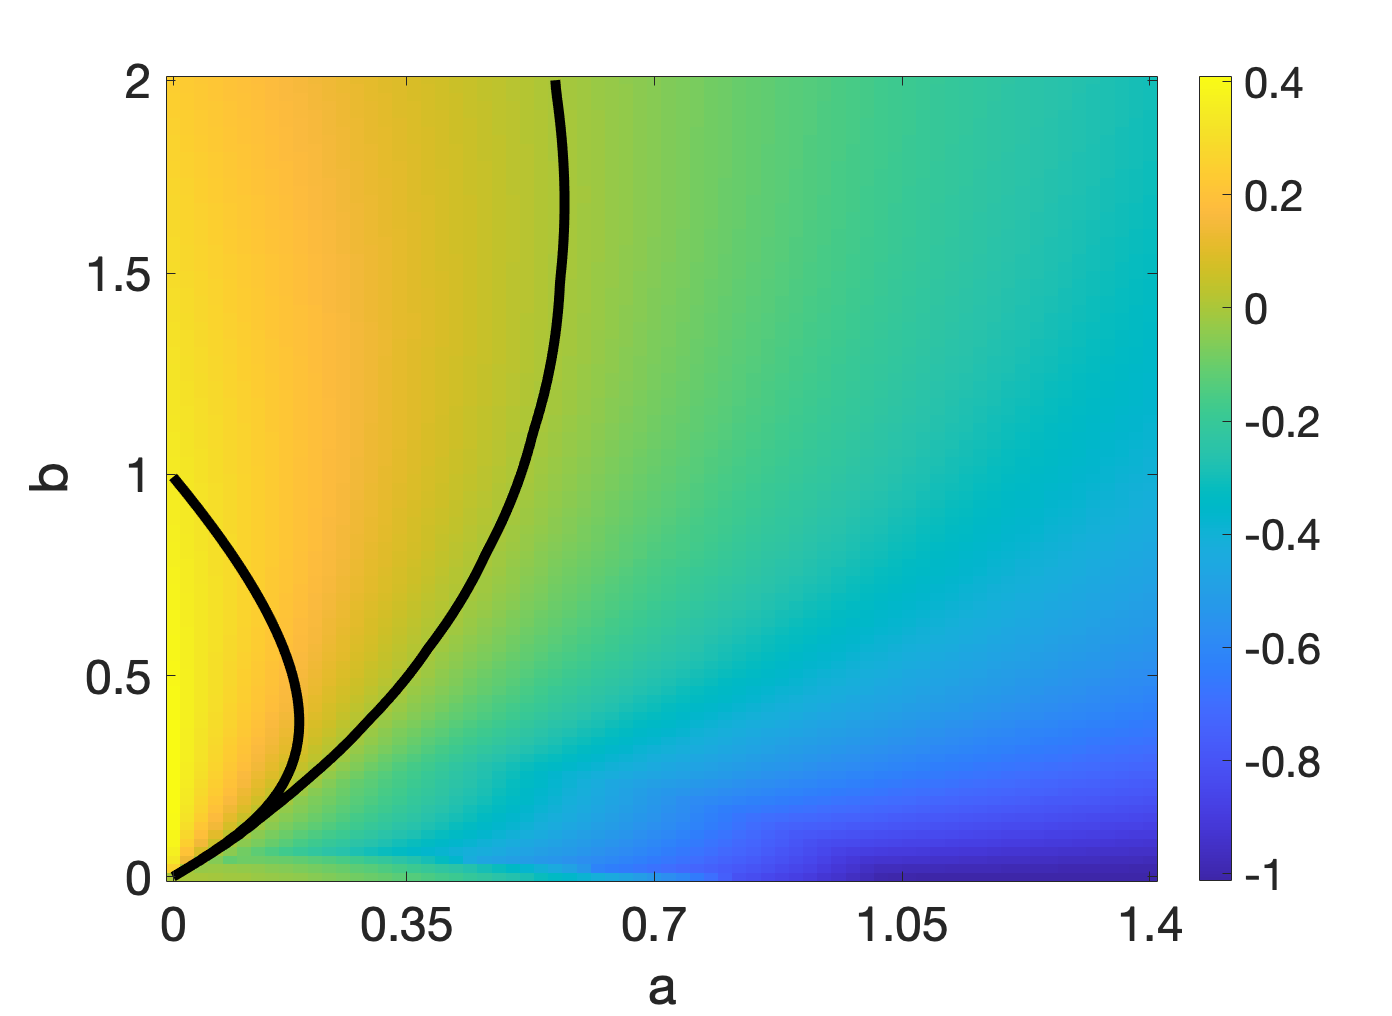
\includegraphics[width=7cm,height=4.75cm]{distbif3.png}
%         \caption{$\tau=0.2$.}
%         \label{}
%     \end{subfigure}
%     \hfill
%     \begin{subfigure}[t]{0.45\textwidth}
%         \centering
%         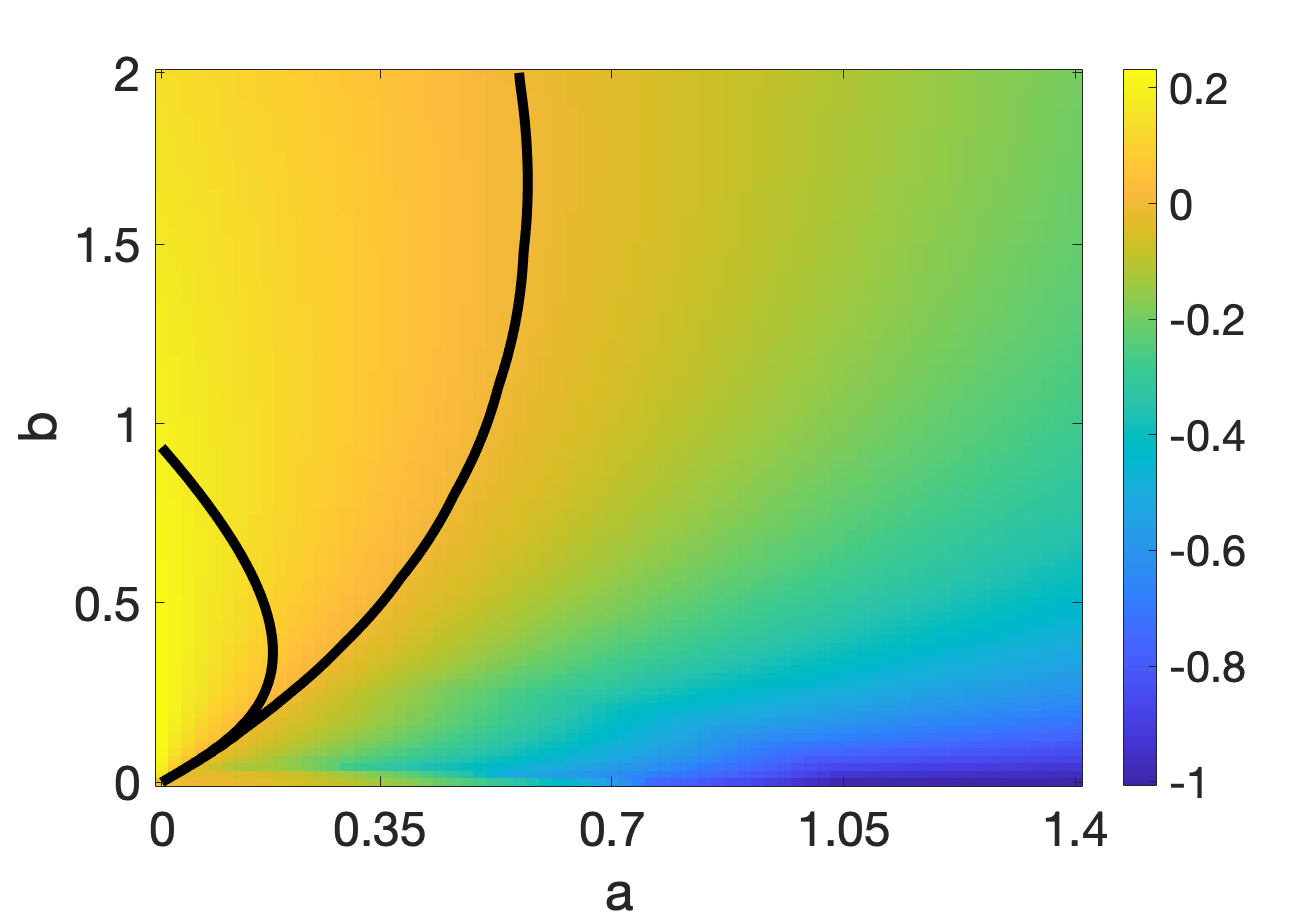
\includegraphics[width=7cm,height=4.75cm]{distbif4.png}
%         \caption{$\tau=0.5$}
%         \label{}
%     \end{subfigure}
%     \caption{Bifurcation diagrams produced by solving \eqref{characfix} (fixed delay characteristic equation) for $\tau=0.2,0.5$ and $\epsilon^2=0.01$, on a domain length $L^2=9/2$.}
%     \label{fig:distheat2}
% \end{figure}

Observing the results in table \ref{tab:tab1}, the largest absolute difference in $\max_k(\Re(\lambda_k))$ for all $\sigma$, $\tau$ and $\epsilon^2$ considered, across the parameter space $(a,b)\in[0,1.4]\times[0,2]$ is $O(10^{-3})$. We therefore expect that for all $(a,b)\in[0,1.4]\times[0,2]$,
using a symmetric Gaussian distribution centred at some mean $\tau$, for small $\tau$, will not significantly effect the time-taken until pattern formation compared to the fixed delay case, independent of the standard deviation $\sigma$ of the distribution. We remark here that absolute differences were considered rather than relative differences, due to the effects of catastrophic cancelling. We numerically confirm these results for varying $\epsilon^2$, $\tau$ and $\sigma$, considering larger delays up to $\tau=16$.

\begin{table}[H]
\centering
\begin{tabular}{lrrrr}
\hline
\multicolumn{2}{c}{Parameters Used}    & $\sigma_{\max}\times0.99$ & $\sigma_{\max}\times0.2\ $ & $\sigma_{\max}\times0.1\ $ \\ \hline
$\epsilon^2=0.001$ & \textbf{$\tau=0.2$} & $0.0010$                           & $4.2\times10^{-5}$                & $1.1\times10^{-5}$                \\
$\epsilon^2=0.001$ & $\tau=1.0$          & $0.0078$                           & $3.3\times10^{-4}$                & $8.2\times10^{-5}$                \\
$\epsilon^2=0.01$  & \textbf{$\tau=0.2$} & $0.0025$                           & $9.4\times10^{-5}$                & $2.3\times10^{-5}$                \\
$\epsilon^2=0.01$  & \textbf{$\tau=0.5$} & \textbf{$0.0076$}                  & $2.6\times10^{-4}$                & $6.4\times10^{-5}$               \\ \hline
\end{tabular}
\caption{Table showing $\max_{(a,b)}$ of absolute difference of $\max_k(\Re(\lambda_k))$ between distributed delay cases and fixed delay case, across the $(a,b)\in[0,1.4]\times[0,2]$ parameter space, for multiple $\tau$ and $\epsilon^2$ values. $L^2=9/2$ used. Results displayed to $2s.f.$}
\label{tab:tab1}
\end{table}

\subsection{Numerical Results}\label{section:distsim}
Numerical simulations are shown here to verify the linear theory presented in section \ref{section:distlin}. We first confirm that the results obtained in figures \ref{fig:p2} and \ref{fig:p3} are accurate, namely that we find pattern formation for $(a,b)=(0.1,0.9)$ but not for $(a,b)=(0.4,0.4)$, independent of the $\tau\in[0,1]$ and $\sigma$ values considered. We also verify our main result, that modelling time delay as a symmetric Gaussian distribution will not quantitatively change the results seen from that of a fixed delay, independent of the $\sigma$ used. Figures \ref{fig:testdist1} and \ref{fig:testdist2} show the numerical solutions for $(a,b)=\{(0.1,0.9),(0.4,0.4)\}$ for $\tau=1$ and varying $\sigma$. Further numerical results with different $\tau$ and $\sigma$ values can be found in appendix \ref{section:appB}. Initial conditions were set as $\text{IC}_2$, as defined in \eqref{firstic}.

\begin{figure}[H]
    \centering
    \begin{subfigure}[t]{0.45\textwidth}
        \centering
        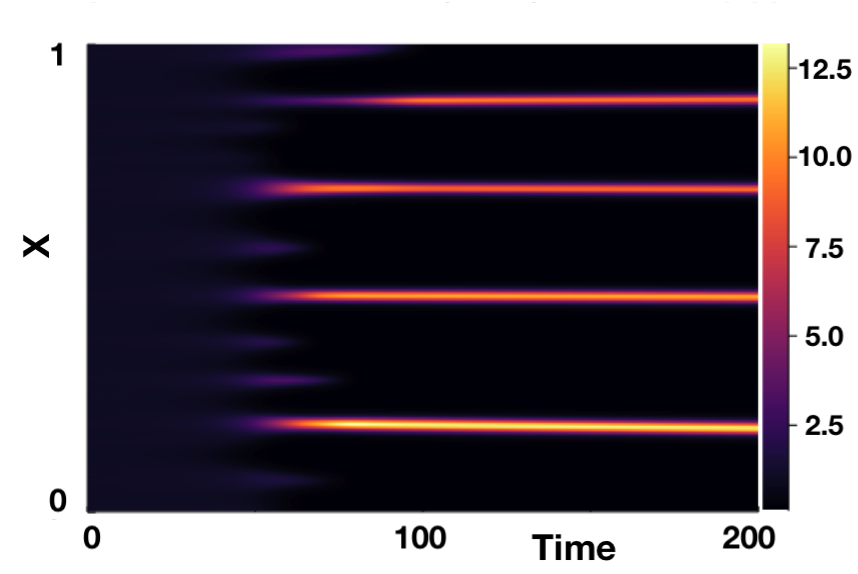
\includegraphics[width=7cm,height=5cm]{distp1sig1.png}
        \caption{Numerical solution with $\tau=1$ and $\sigma=\sigma_{max}\times0.99$.}
        \label{}
    \end{subfigure}
    \hfill
    \begin{subfigure}[t]{0.45\textwidth}
        \centering
        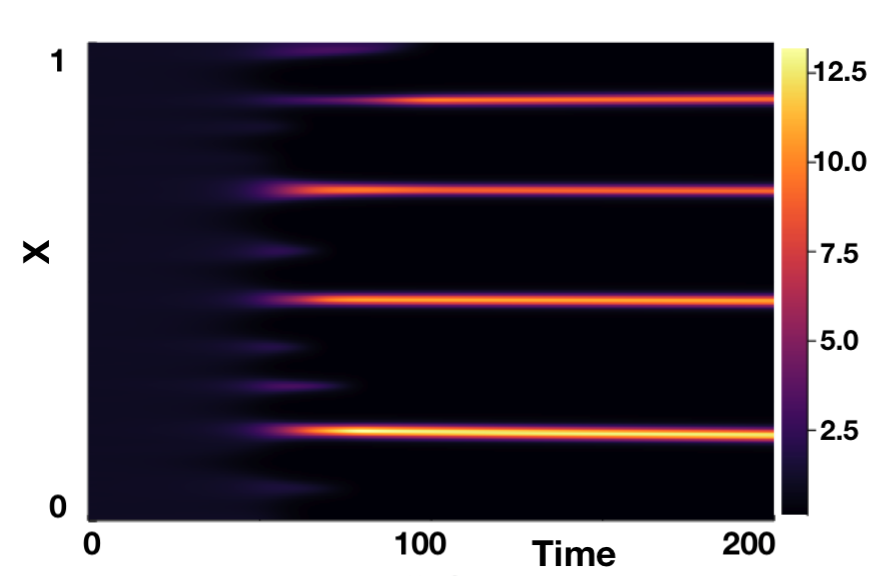
\includegraphics[width=7cm,height=5cm]{distp1sig2.png}
        \caption{Numerical solution with $\tau=1$ and $\sigma=\sigma_{max}\times0.1$.}
        \label{}
    \end{subfigure}
    \caption{Numerical solutions produced for $(a,b)=(0.1,0.9)$ with $\tau=1$ and $\sigma=\sigma_{max}\times0.99, \sigma_{max}\times0.1$. We use $L^2=9/2$ and $\epsilon^2=0.001$.
    Boundary conditions given by \eqref{neumannbc} and initial conditions by \eqref{firstic}. We see pattern formation, as predicted from linear theory.}
    \label{fig:testdist1}
\end{figure}

\begin{figure}[H]
    \centering
    \begin{subfigure}[t]{0.45\textwidth}
        \centering
        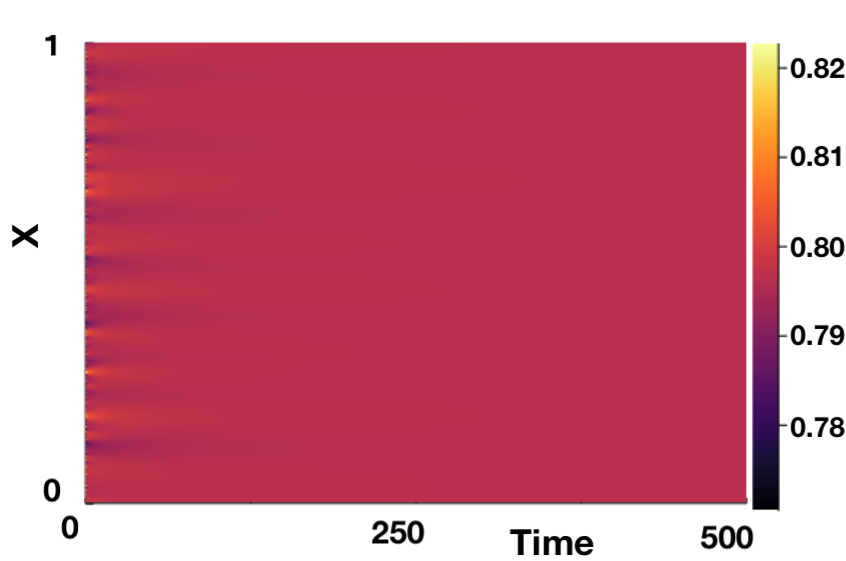
\includegraphics[width=7cm,height=5cm]{distp2sig1.png}
        \caption{Numerical solution with $\tau=1$ and $\sigma=\sigma_{max}\times0.99$.}
        \label{}
    \end{subfigure}
    \hfill
    \begin{subfigure}[t]{0.45\textwidth}
        \centering
        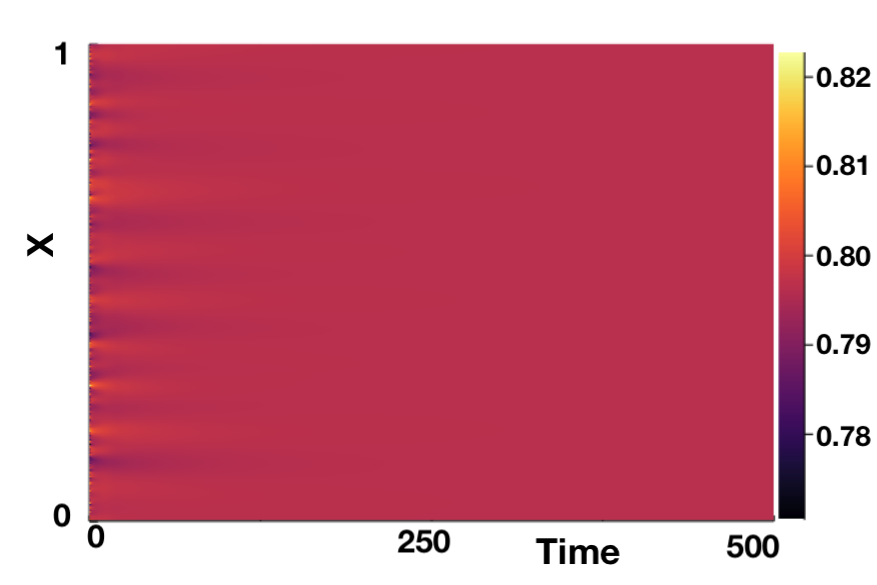
\includegraphics[width=7cm,height=5cm]{distp2sig2.png}
        \caption{Numerical solution with $\tau=1$ and $\sigma=\sigma_{max}\times0.1$.}
        \label{}
    \end{subfigure}
    \caption{Numerical solutions produced for $(a,b)=(0.4,0.4)$ with $\tau=1$ and $\sigma=\sigma_{max}\times0.99, \sigma_{max}\times0.1$. We use $L^2=9/2$ and $\epsilon^2=0.001$. Boundary conditions given by \eqref{neumannbc} and initial conditions by \eqref{firstic}. We see no pattern formation, as predicted from linear theory.}
    \label{fig:testdist2}
\end{figure}
Figures \ref{fig:distres1} and \ref{fig:distres2} show the numerical solution using $(a,b)=(0.1,0.9)$ for $\tau=1,16$ and varying $\sigma$, each compared with the appropriate fixed delay case. The results indicated that the onset of patterning, and the type of pattern we see, is independent of $\sigma$ used. Further numerical solution for different $(a,b)$ and $\epsilon^2$ verifying this claim can be found in appendix \ref{section:appB}.

\begin{figure}[H]
    \centering
    \begin{subfigure}[t]{0.32\textwidth}
        \centering
        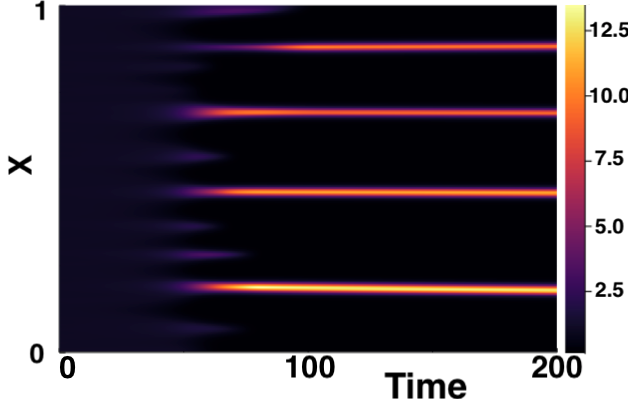
\includegraphics[width=5cm,height=4.5cm]{ic21.png}
        \caption{Fixed delay model given by \eqref{fixed2}.}
        \label{}
    \end{subfigure}
    \hfill
    \begin{subfigure}[t]{0.32\textwidth}
        \centering
        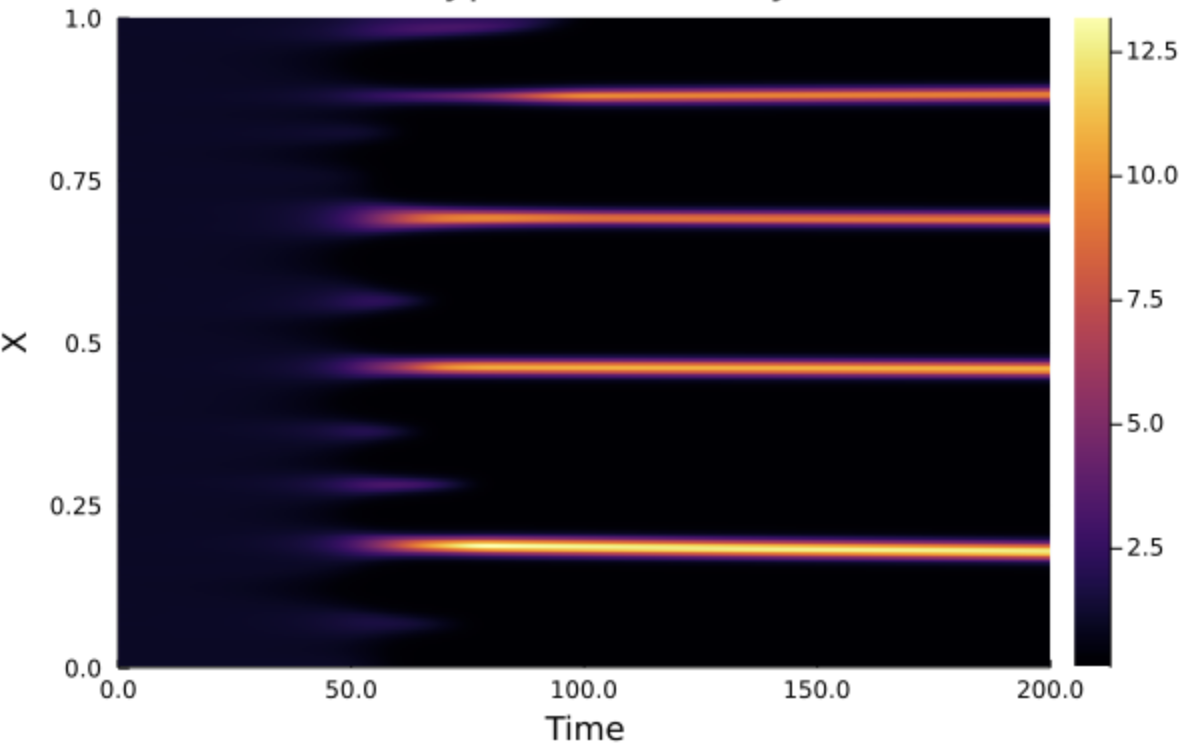
\includegraphics[width=5cm,height=4.5cm]{distt1sigmax.png}
        \caption{Distributed delay model, \eqref{symmod}, with $\sigma=\sigma_{\max}\times0.99$.}
        \label{}
    \end{subfigure}
    \hfill
    \begin{subfigure}[t]{0.32\textwidth}
        \centering
        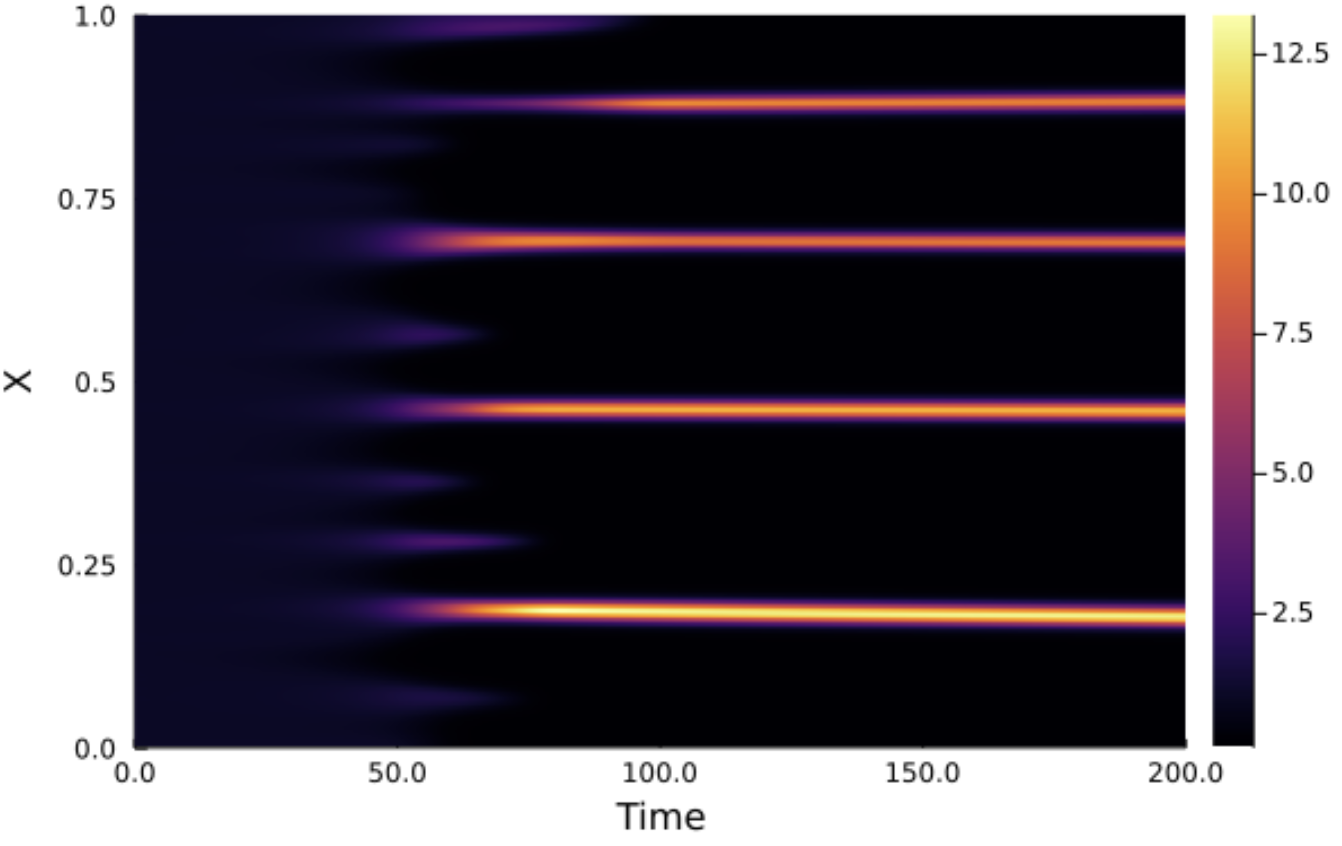
\includegraphics[width=5cm,height=4.5cm]{distt1sig10.png}
        \caption{Distributed delay model, \eqref{symmod}, with $\sigma=\sigma_{\max}\times0.1$.}
        \label{}
    \end{subfigure}
    \caption{Numerical simulations showing comparison of fixed delay case vs distributed delay case for $\tau=1$. Boundary conditions given by \eqref{neumannbc} and initial conditions by \eqref{firstic}. $(a,b)=(0.1,0.9)$, $\epsilon^2=0.001$, $L^2=9/2$. }
    \label{fig:distres1}
\end{figure}
\begin{figure}[H]
    \centering
    \begin{subfigure}[t]{0.32\textwidth}
        \centering
        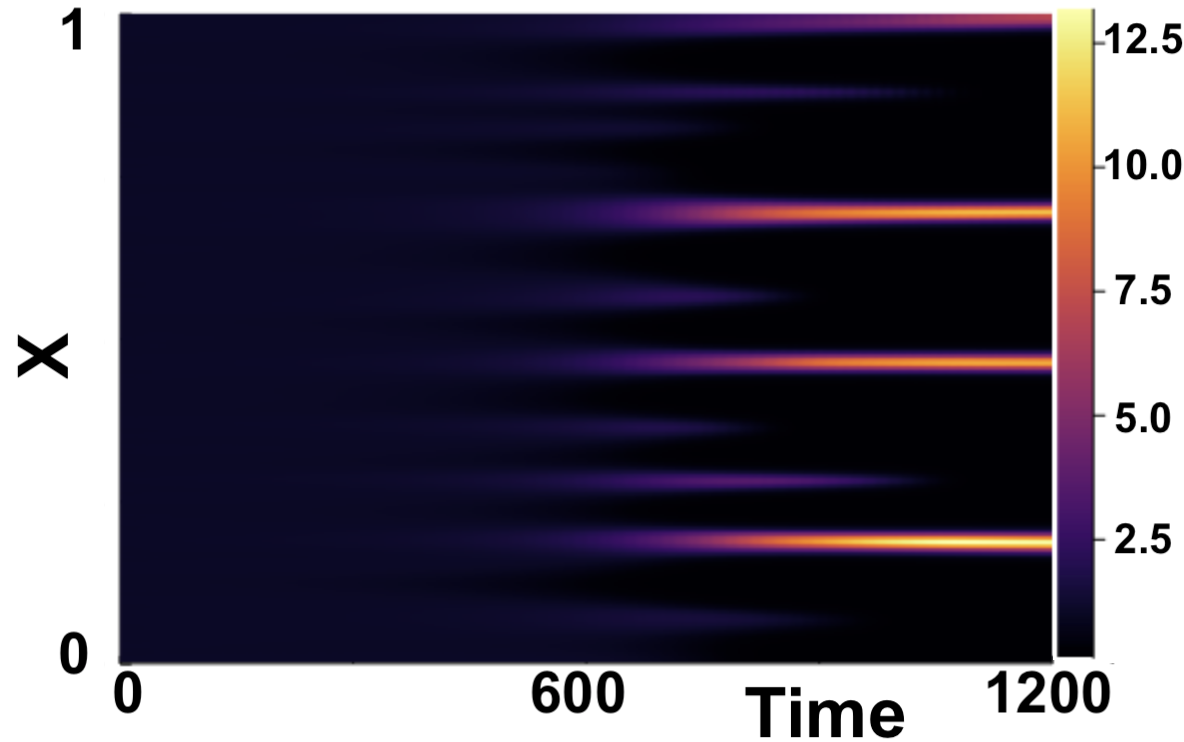
\includegraphics[width=5cm,height=4.5cm]{distt16sig10.png}
        \caption{Fixed delay model given by \eqref{fixed2}.}
        \label{}
    \end{subfigure}
    \hfill
    \begin{subfigure}[t]{0.32\textwidth}
        \centering
        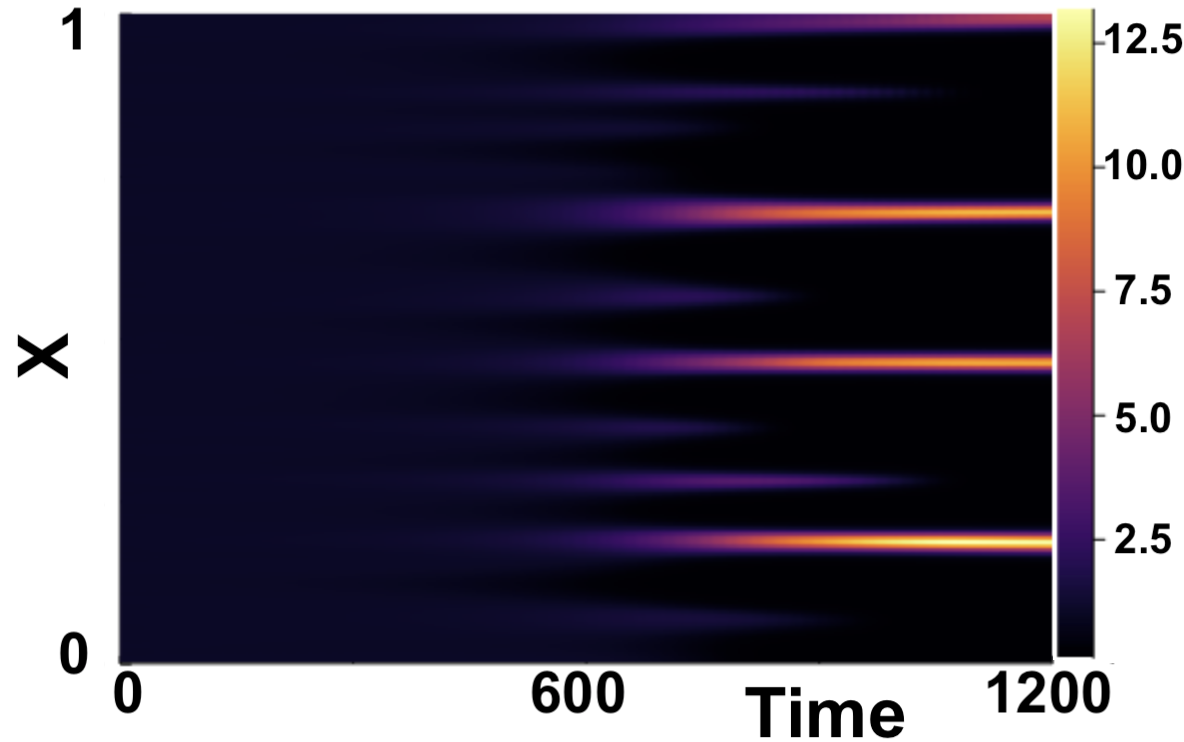
\includegraphics[width=5cm,height=4.5cm]{distt16sig10.png}
        \caption{Distributed delay model, \eqref{symmod}, with $\sigma=\sigma_{\max}\times0.99$.}
        \label{}
    \end{subfigure}
    \hfill
    \begin{subfigure}[t]{0.32\textwidth}
        \centering
        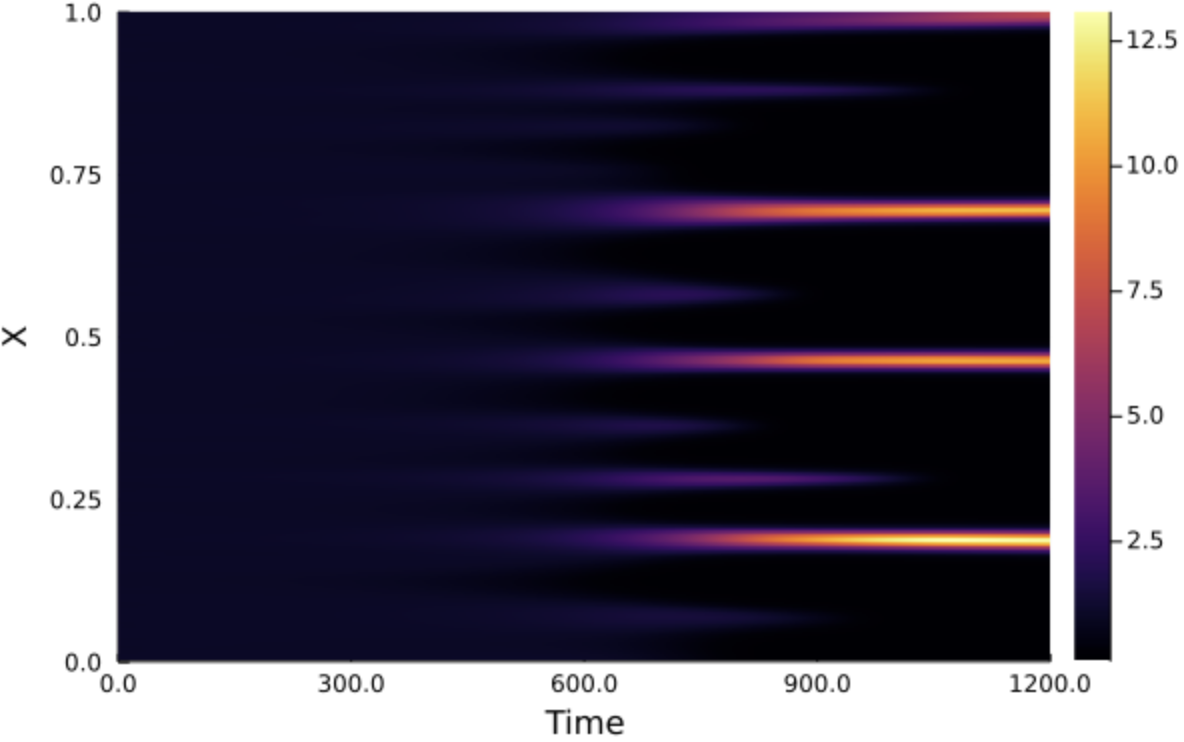
\includegraphics[width=5cm,height=4.5cm]{distt16sigmax.png}
        \caption{Distributed delay model, \eqref{symmod}, with $\sigma=\sigma_{\max}\times0.1$.}
        \label{}
    \end{subfigure}
    \caption{Numerical simulations showing comparison of fixed delay case vs distributed delay case for $\tau=16$. Boundary conditions given by \eqref{neumannbc} and initial conditions by \eqref{firstic}. $(a,b)=(0.1,0.9)$, $\epsilon^2=0.001$, $L^2=9/2$.}
    \label{fig:distres2}
\end{figure}
% Parameter set 2
%\begin{figure}[H]
%    \centering
%    \begin{subfigure}[t]{0.32\textwidth}
%        \centering
%        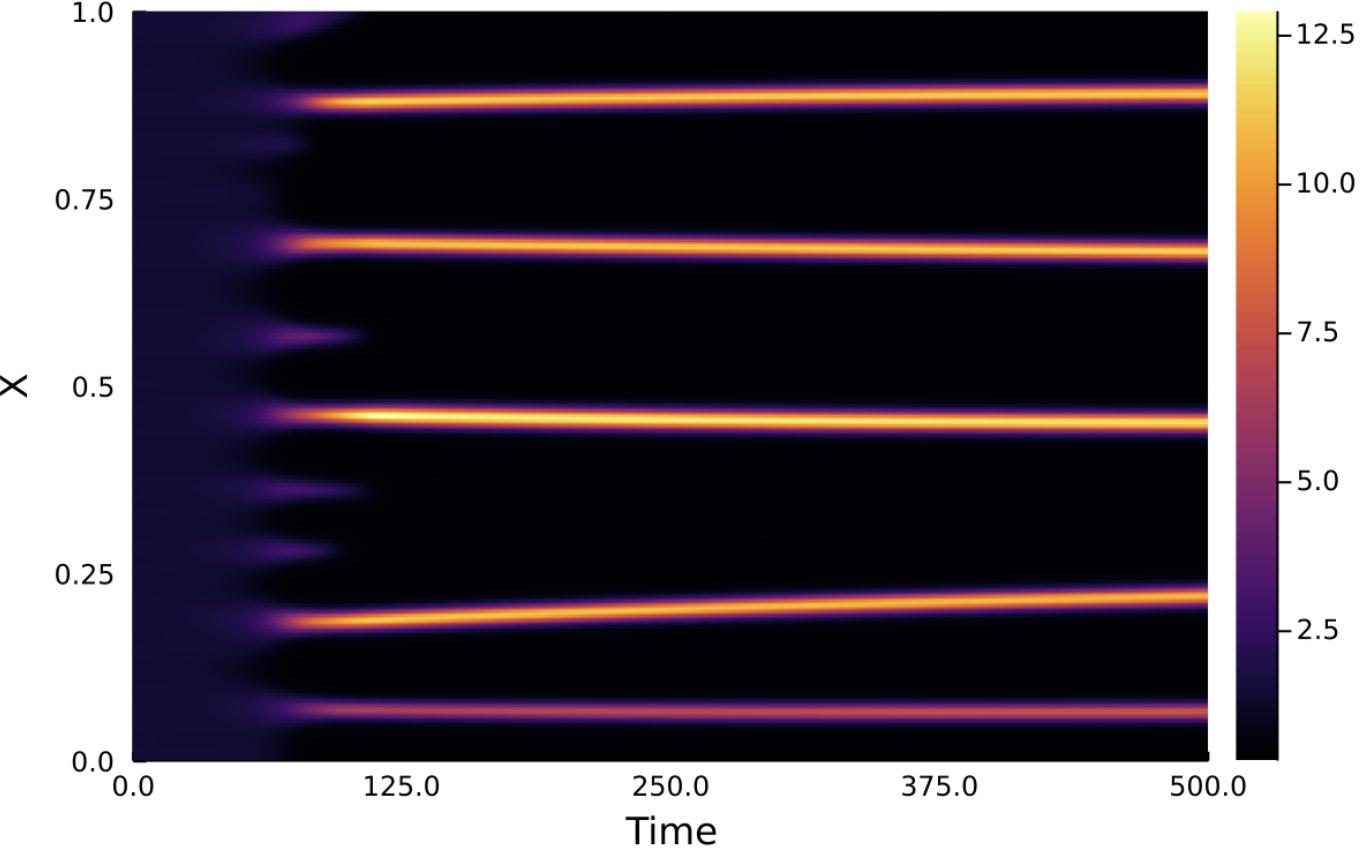
\includegraphics[width=5cm,height=4.5cm]{dist2t1sigmax.png}
%        \caption{Fixed delay model given by \eqref{fixed2}.}
%        \label{}
%    \end{subfigure}
%    \hfill
%    \begin{subfigure}[t]{0.32\textwidth}
%        \centering
%        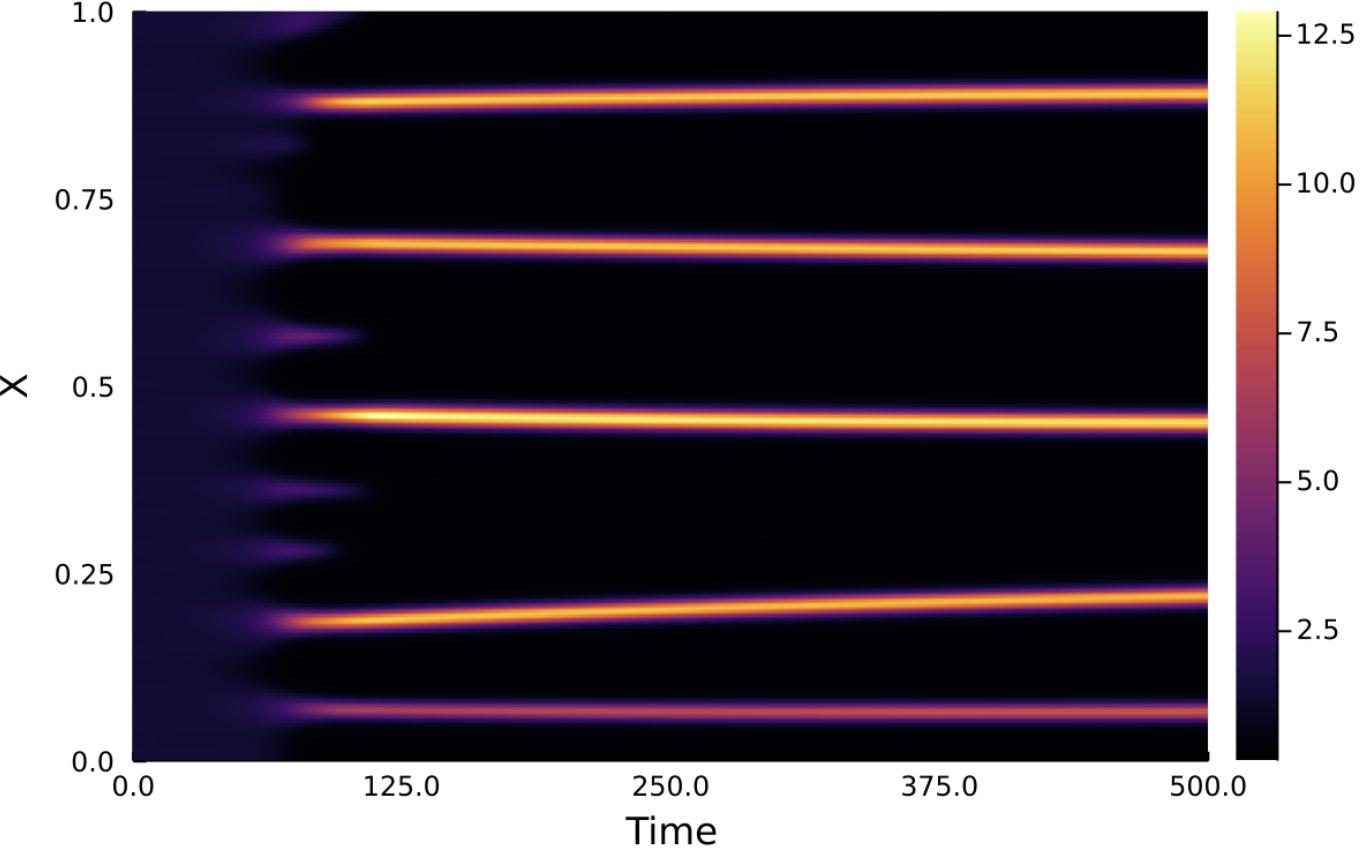
\includegraphics[width=5cm,height=4.5cm]{dist2t1sigmax.png}
%        \caption{Distributed delay model, \eqref{symmod}, with $\sigma=\sigma_{\max}\times0.99$.}
%        \label{}
%    \end{subfigure}
%    \hfill
%    \begin{subfigure}[t]{0.32\textwidth}
%        \centering
%        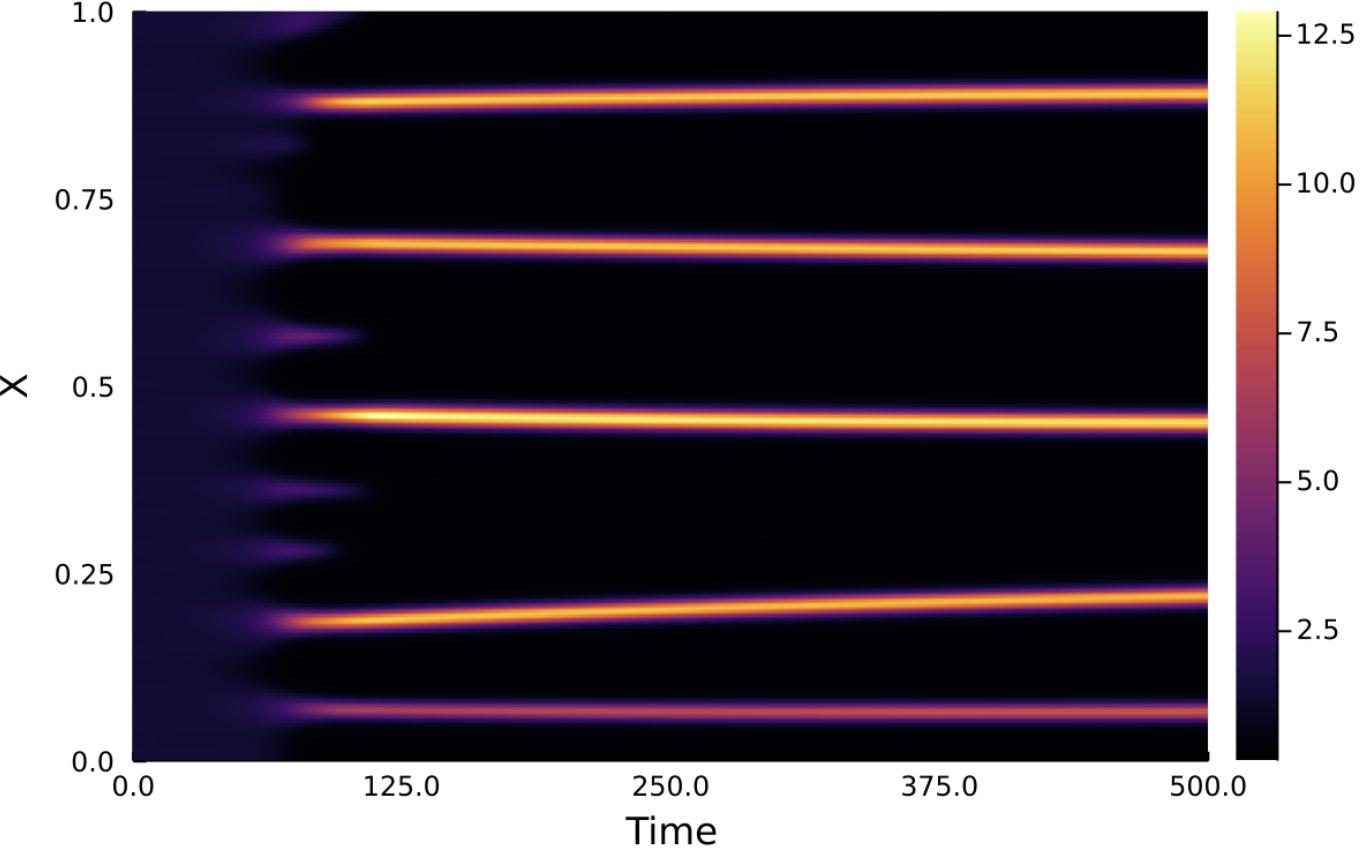
\includegraphics[width=5cm,height=4.5cm]{dist2t1sigmax.png}
%        \caption{Distributed delay model, \eqref{symmod}, with $\sigma=\sigma_{\max}\times0.1$.}
%        \label{}
%    \end{subfigure}
%    \caption{Numerical simulations showing comparison of fixed delay case vs distributed delay case for $\tau=1$. Boundary conditions given by \eqref{neumannbc} and initial conditions by \eqref{firstic}. $(a,b)=(0.3,1.2)$, $\epsilon^2=0.001$, $L^2=9/2$.}
%    \label{fig:distres3}
%\end{figure}
% \begin{figure}[H]
%     \centering
%     \begin{subfigure}[t]{0.32\textwidth}
%         \centering
%         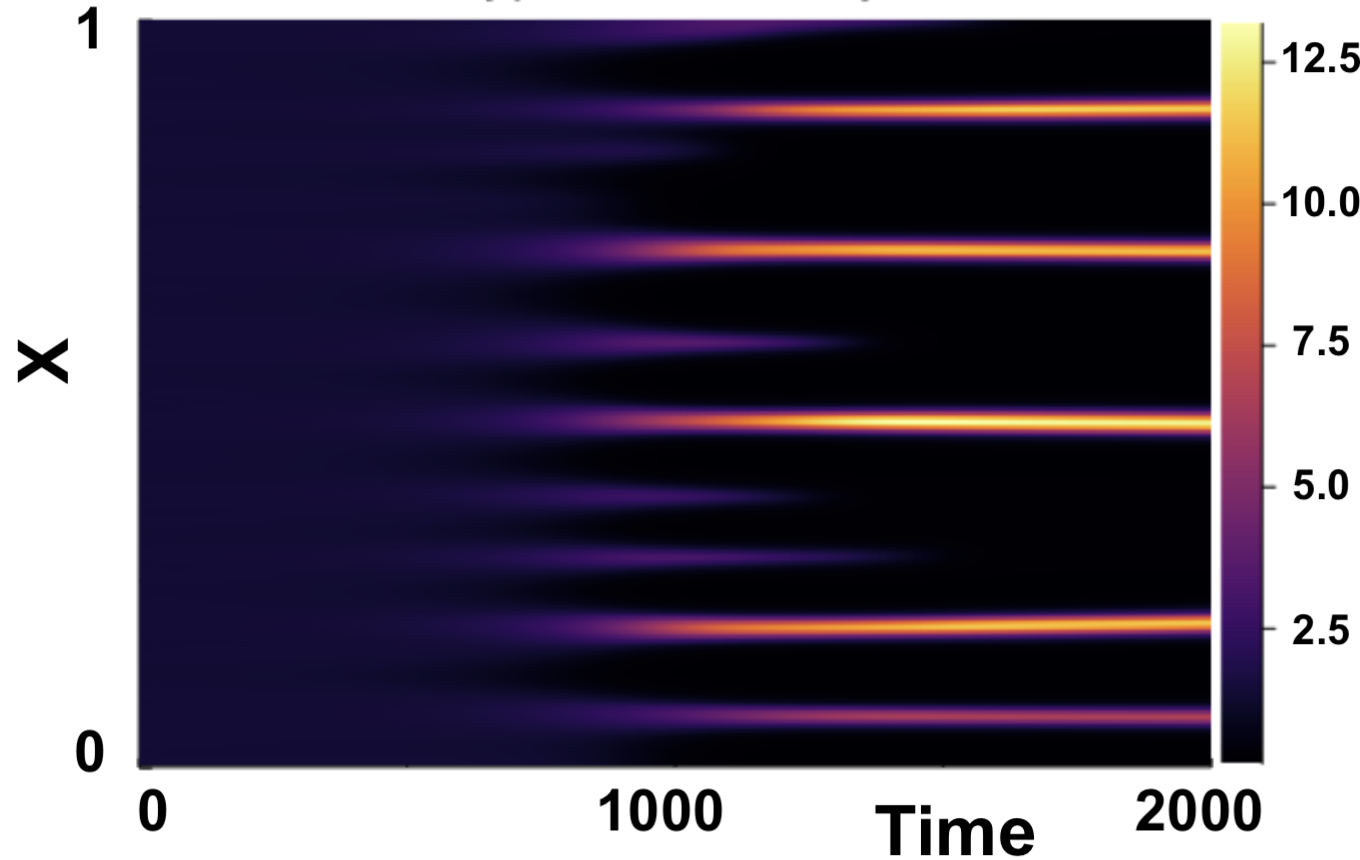
\includegraphics[width=5cm,height=4.5cm]{dist2t16sigmax.png}
%         \caption{Fixed delay model given by \eqref{fixed2}.}
%         \label{}
%     \end{subfigure}
%     \hfill
%     \begin{subfigure}[t]{0.32\textwidth}
%         \centering
%         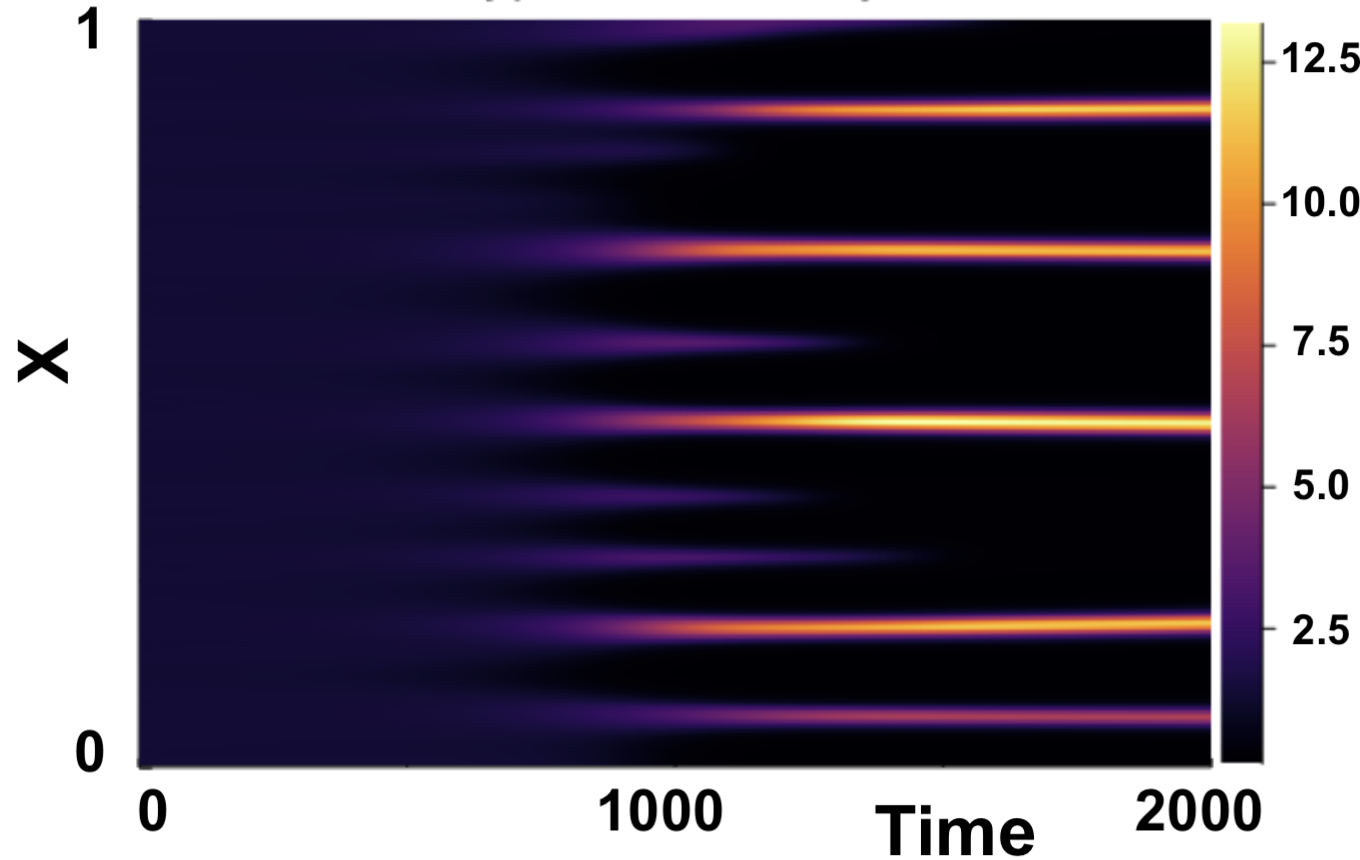
\includegraphics[width=5cm,height=4.5cm]{dist2t16sigmax.png}
%         \caption{Distributed delay model, \eqref{symmod}, with $\sigma=\sigma_{\max}\times0.99$.}
%         \label{}
%     \end{subfigure}
%     \hfill
%     \begin{subfigure}[t]{0.32\textwidth}
%         \centering
%         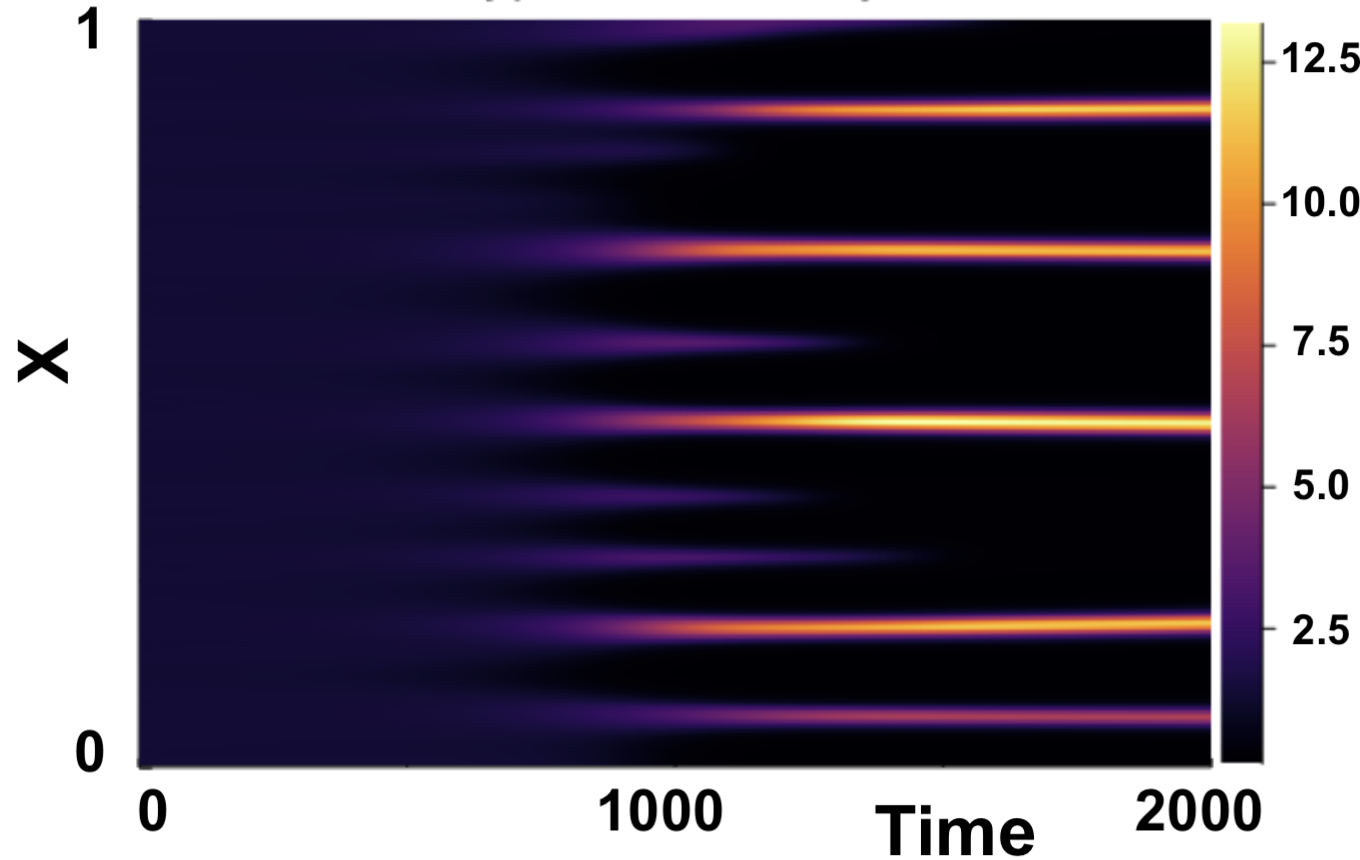
\includegraphics[width=5cm,height=4.5cm]{dist2t16sigmax.png}
%         \caption{Distributed delay model, \eqref{symmod}, with $\sigma=\sigma_{\max}\times0.1$.}
%         \label{}
%     \end{subfigure}
%     \caption{Numerical simulations showing comparison of fixed delay case vs distributed delay case for $\tau=16$. Boundary conditions given by \eqref{neumannbc} and initial conditions by \eqref{firstic}. $(a,b)=(0.3,1.2)$, $\epsilon^2=0.001$, $L^2=9/2$.}
%     \label{fig:distres4}
%\end{figure}




\section{An Asymmetric Distribution}
\subsection{Introduction}
The results in section \ref{section:symmetric} suggest that using a symmetric Gaussian distribution does not have a quantitative effect on the results seen compared to that of the fixed delay case, and thus does not remedy the increased time-to-pattern problems caused by introducing a fixed time delay. We therefore consider how an asymmetric distribution, specifically a skewed truncated Gaussian distribution, affects the results compared to that of a fixed delay. Using the results in \cite{skewed}, and letting $\textbf{p}=(\mu,\omega,\rho)$, the probability density function of the skewed truncated Gaussian distribution, $k(s;\mu,\omega,\rho)$, for some location $\mu$ and scaling $\omega$, is given by
\begin{equation}
    k(s;\mu,\omega,\rho)=\frac{\Psi_c}{\omega}\sqrt{\frac{2}{\pi}}\exp\left(-\frac{1}{2}\left(\frac{s-\mu}{\omega}\right)^2\right)\phi\left(\rho\frac{s-\mu}{\omega}\right),
\end{equation}
where $\phi(x)$ is the same as defined \eqref{phi}. The new parameter $\rho$ is used to denote the skew factor. The distribution is negatively skewed for $\rho<0$ and postively skewed for $\rho>0$. Finally, we have that $\Psi_c$ is the truncation scaling constant. This is given as
\begin{equation}
    \Psi_c=\frac{1}{F\left(\frac{b-\mu}{\omega},\rho\right)-F\left(\frac{a-\mu}{\omega},\rho\right)},
\end{equation}
with $F(x,\rho)$ the cdf of a skewed Gaussian distribution, described by
\begin{equation}
    F(x,\rho)=\phi(x)-2T(x,\rho).
\end{equation}
The function $T(x,\rho)$ denotes the Owen's T function \cite{owenst} and is written as an integral in the form
\begin{equation}
    T(x,\rho)=\frac{1}{2\pi}\int_0^\rho\frac{e^{-\frac{1}{2}x^2(1+s^2)}}{1+s^2}\ \text{d}s\quad -\infty<x,\rho<\infty.
\end{equation}
In the computational implementation of the skewed truncated Gaussian pdf, the integral $T(x,\rho)$ is resolved numerically using the composite Simpson's rule (with a large number of discretisation points).

We note now that since the distribution is skewed, the parameters $\mu$ and $\omega$ no longer denote the mean and standard deviation of the distribution, but solely the location and scale of the distribution. To compare how the skewed distribution affects the onset of patterning compared to that of the fixed delay case, we require the mean of the skewed distribution, $\tau$, which is given by
\begin{equation}\label{anmean}
    \tau=\int_a^bs\ k(s;\mu,\omega,\rho)\ \ \text{d}s.
\end{equation}
Deriving results from \cite{skewed}, the mean of the skewed truncated Gaussian distribution is computed as
\begin{equation}\label{computetau}
\tau=\mu+\omega\Psi_c\left[k(a;\mu,\omega,\rho)-k(b;\mu,\omega,\rho)+\frac{2\rho}{\hat{\rho}\sqrt{2\pi}}\left(\phi\left(\hat{\rho}\frac{b-\mu}{\omega}\right)-\phi\left(\hat{\rho}\frac{a-\mu}{\omega}\right)\right)\right].
\end{equation}
The scalar $\hat{\rho}$ is given as $\hat{\rho}=\left(1+\rho^2\right)^{1/2}$. The additional mathematical details for how \eqref{computetau} was obtained can be found in Appendix \ref{section:appA}.

Throughout this section, the integration limits were set to $a=\mu-3\omega$, $b=\mu+3\omega$, where $\omega$ was chosen such that $\omega<\omega_{\max}$, with $\omega_{\max}=\frac{\mu}{3}$ to ensure only positive time delays were considered.
\subsection{Linear Analysis}\label{section:linanalskew}
Conducting an analogous linear analysis to that of the symmetric distibuted delay case, we find that the characterstic equation when a skewed distribution is being used is given as
\begin{equation}\label{characskew}
  \mathcal{D}_k=\lambda_k^2+\alpha_k\lambda_k+\beta_k+(\gamma_k\lambda_k+\delta_k)\hat{E}_k=0,
\end{equation}
where $\alpha_k$, $\beta_k$, $\gamma_k$ and $\delta_k$ are the same coefficients as defined in \eqref{characcoeff}, for the symmetric distribution case. The difference is in expression $\hat{E}_k$, which is given by
\begin{equation}\label{Ehat}
    \begin{split}
\hat{E}_k&=\int_a^bk(s;\mu,\omega,\rho)e^{-\lambda_k s}\ \text{d}s\\
&=\frac{\Psi_c}{\omega\sqrt{2\pi}}\int_a^b\left(1+\text{erf}\left(\rho\frac{s-\mu}{\omega\sqrt{2}}\right)\right)\exp\left(-\frac{1}{2}\left(\frac{s-\mu}{\omega}\right)^2-\lambda_ks\right)\ \text{d}s.
    \end{split}
\end{equation}
This integral cannot be evaluated explicitly using standard mathematical functions\footnote{The integral was attempted to be evaluated via Wolframalpha}, but can however be evaluated numerically using a quadrature rule. We use the composite Simpson's rule, with a large number of discretisation points. This allows roots of the characteristic eqution \eqref{characskew} to be solved for.

Here we present results of the $\max_k(\Re(\lambda_k))$ for varying $\tau$ with a skewed distribution. Namely, we show that for a small mean $\tau$, the skew, positive or negative, does not significantly effect the $\max_k(\Re(\lambda_k))$. We note that, for a given $\rho$, all of the terms on the right hand side of \eqref{computetau}, namely $\omega$, $\Psi_c$,  and $k(s;\mu,\omega,\rho)$, can be written explicitly in terms of $\mu$. Equation \eqref{computetau} can therefore be solved implicitly for $\mu(\tau)$, for a given $\tau$, using the \textit{fzero} command in MATLAB. For a given $\rho$, and each found $\mu$, we compute $\max_k(\Re(\lambda_k))$ by solving for roots of the characterstic equation \eqref{characskew}. In figure \ref{fig:dispskew}, we plot $\max_k(\Re(\lambda_k))$ against $\tau\in[0,0.8]$ for skew parameter values of $\rho=-10,10$, and $\omega=\omega_{\max}\times0.99$, with two different $(a,b)$ parameter sets. A plot of $\max_k(\Re(\lambda_k))$ for the fixed delay case is also added for comparison in each case.

\begin{figure}[H]
    \centering
    \begin{subfigure}[t]{0.45\textwidth}
        \centering
        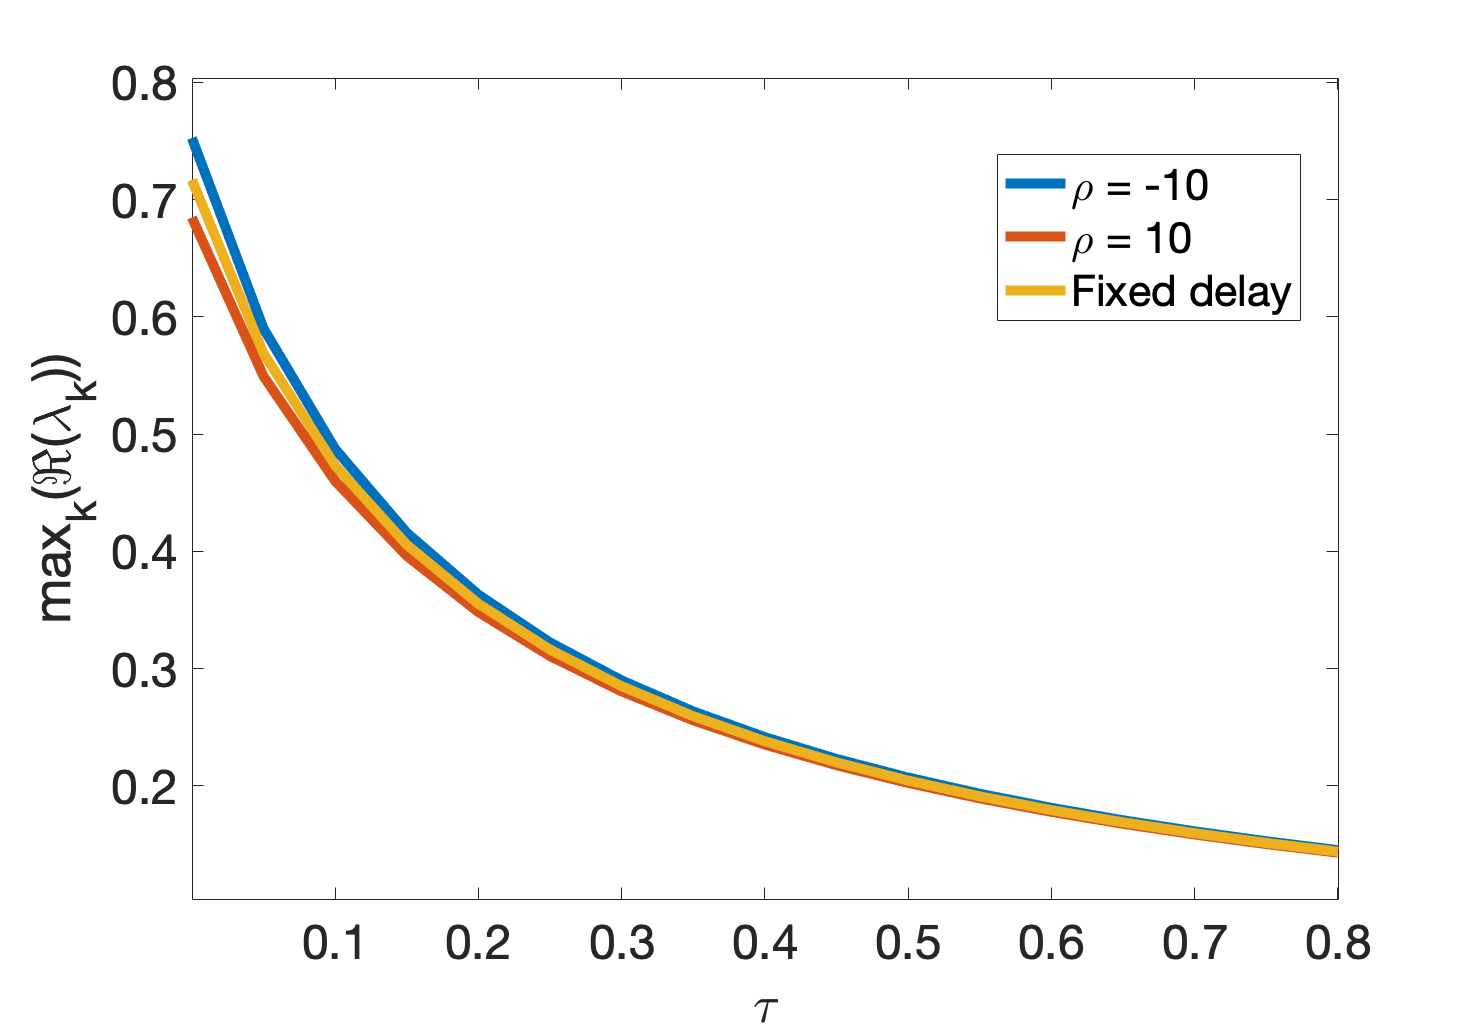
\includegraphics[width=7cm,height=5cm]{dispskew.png}
        \caption{$(a,b)=(0.1,0.9)$.}
        \label{}
    \end{subfigure}
    \hfill
    \begin{subfigure}[t]{0.45\textwidth}
        \centering
        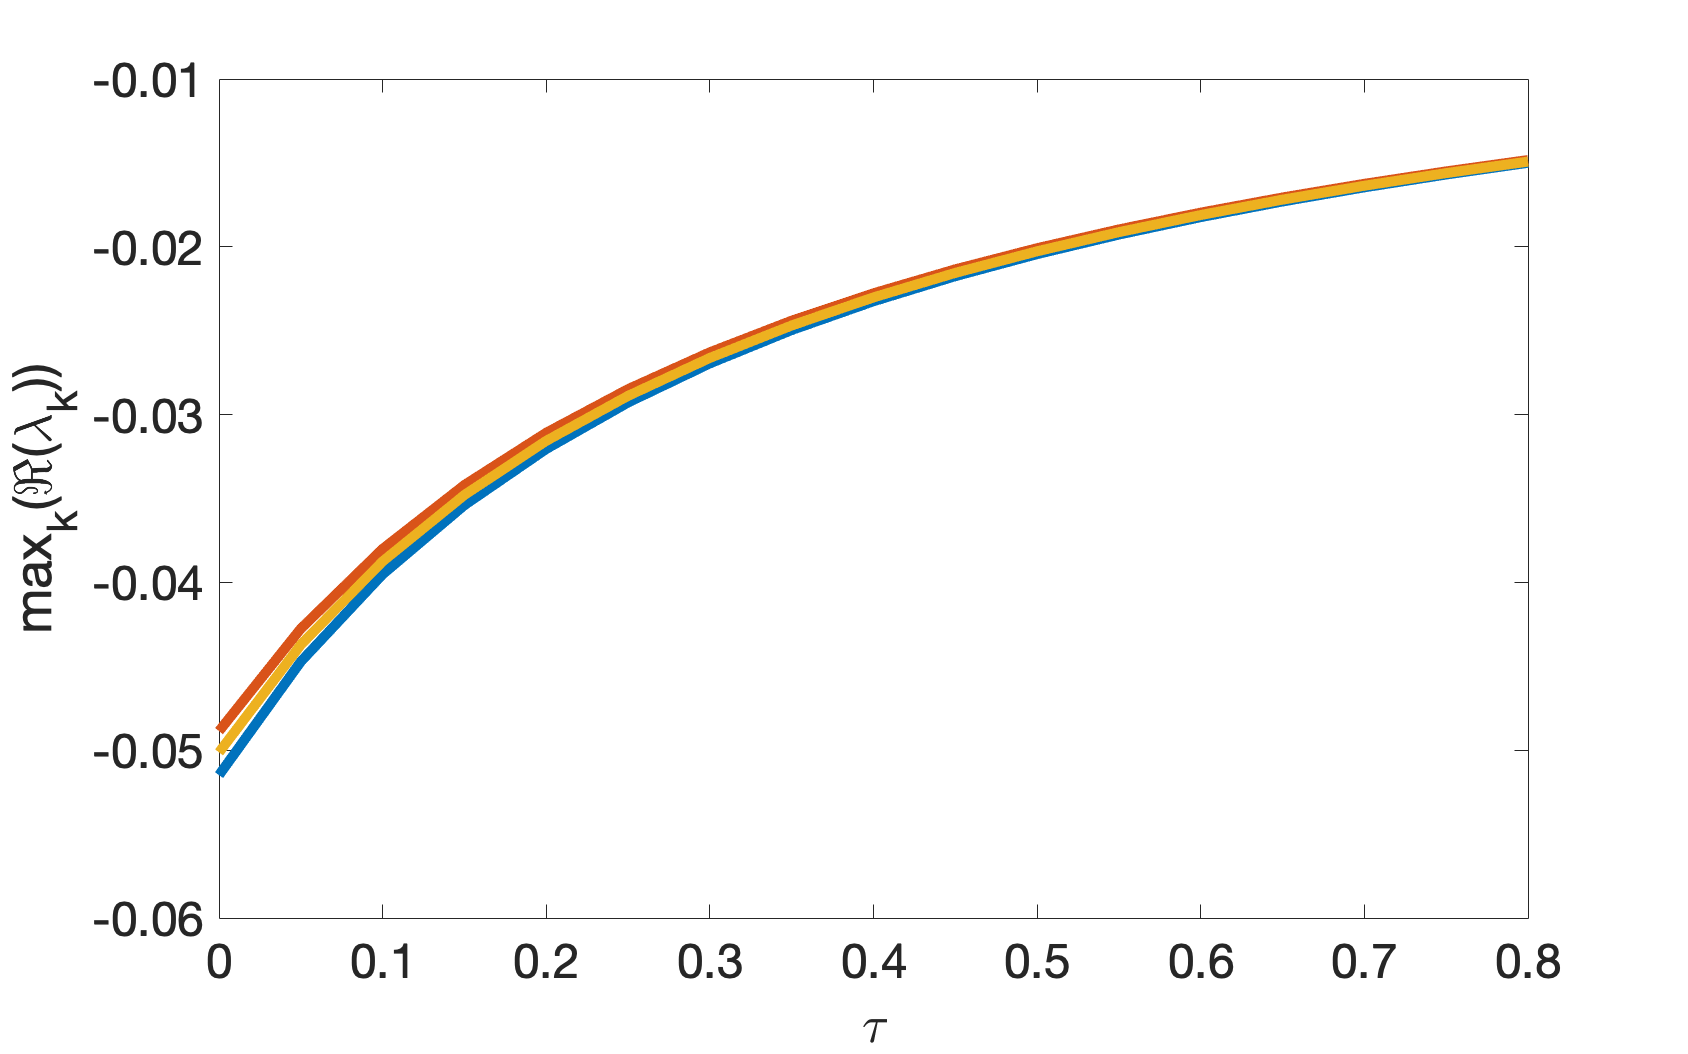
\includegraphics[width=7cm,height=5cm]{dispskew2.png}
        \caption{$(a,b)=(0.4,0.4)$.}
        \label{}
    \end{subfigure}
    \caption{Comparison of $\max_k(\Re(\lambda_k))$ plotted against $\tau\in[0,0.8]$ for $\rho=-10,10$ against fixed delay case. Parameter values $\epsilon^2=0.001$ and $L^2=9/2$ used. $\tau$ varied at regular intervals of $0.05$. $k\in\mathbb{Z}$ ranging over $k\in[0,50]$.}
    \label{fig:dispskew}
\end{figure}
From figure \ref{fig:dispskew} we see that the curves differ very minorly for small $\tau$, with $\rho=-10$ having a slightly higher value of the maximum growth rate, and $\rho=10$ a slightly lower value. The overall effect is very small despite the large skew implemented in the distribution. By comparing the results in figure \ref{fig:dispskew} to those in \ref{fig:p2} and \ref{fig:p3} (dispersion curves for the symmetric distribution vs fixed delay case), we see that the skewed distributions have a larger, but still small, effect on the dispersion curves. We suspect however that these effects are still small enough not to have a significant impact on the timescale on which onset of patterning occurs. Numerical simulations confirming these finding from the linear theory for a small $\tau=0.1$ and $(a,b)=(0.1,0.9)$ can be seen in figure \ref{fig:linskew1}, where we see a very minor varyation in onset of patterning between the $\rho=-10$ and $\rho=10$ cases. Numerical results for further $\tau$ and $(a,b)$ values can be found in appendix \ref{section:appB}.

\begin{figure}[H]
    \centering
    \begin{subfigure}[t]{0.45\textwidth}
        \centering
        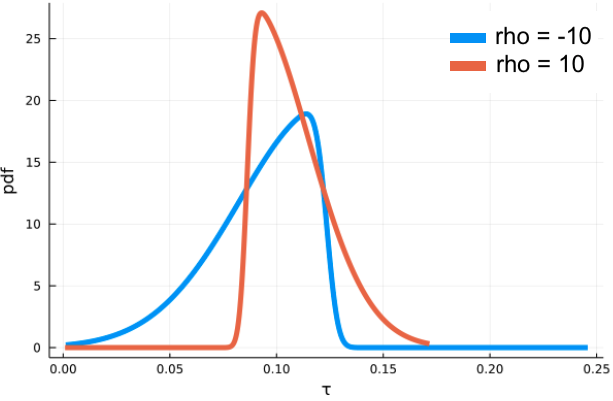
\includegraphics[width=7cm,height=4.75cm]{skewdist.png}
        \caption{pdfs of skewed truncated Gaussian distributions, with $\rho=-10,10$. Both pdfs have mean $\tau=0.1$.}
        \label{}
    \end{subfigure}
    \hfill
    \begin{subfigure}[t]{0.45\textwidth}
        \centering
        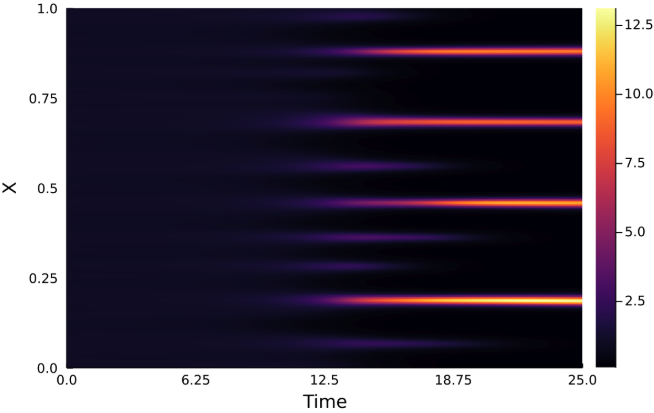
\includegraphics[width=7cm,height=4.75cm]{fixp1.png}
        \caption{Numerical simulation of fixed delay case with $\tau=0.1$.}
        \label{}
    \end{subfigure}
    \hfill
    \begin{subfigure}[t]{0.45\textwidth}
        \centering
        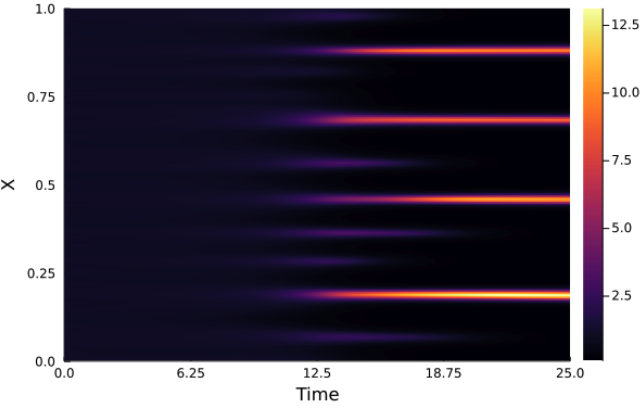
\includegraphics[width=7cm,height=4.75cm]{skewm10.png}
        \caption{Numerical simulation with skewed distribution of $\rho=-10$. Distribution parameters are $\mu=0.124(3.s.f)$ and $\omega=0.0408(3.s.f)$.}
        \label{}
    \end{subfigure}
    \hfill
    \begin{subfigure}[t]{0.45\textwidth}
        \centering
        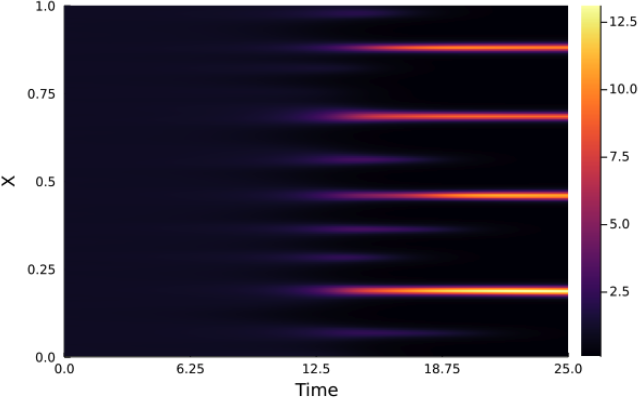
\includegraphics[width=7cm,height=4.75cm]{skew10.png}
        \caption{Numerical simulation with skewed distribution of $\rho=10$. Distribution parameters are $\mu=0.0863(3.s.f)$ and $\omega=0.0285(3.s.f)$.}
        \label{}
    \end{subfigure}
    \caption{Numerical rsesults for $(a,b)=(0.1,0.9)$ with $\rho=-10,10$ and $\tau=0.1$. Parameters $\epsilon^2=0.01$ and $L^2=9/2$. Initial conditions given by \eqref{firstic} and boundary conditions by \eqref{neumannbc}.}
    \label{fig:linskew1}
\end{figure}


\subsection{Numerical Results}

We now look to show through full numerical solutions that for a larger $\tau$ the results we see are consistent with the finding from linear theory for a smaller $\tau$. Namely, we show that using a skewed truncated Gaussian distribution does not have a significant effect on the onset of patterning. Using an analogous methodology as outlined in the previous section \ref{section:linanalskew}, we present results for $\tau=8,16$, and a $\rho=-10,10$ for a fixed parater set $(a,b)=(0.1,0.9)$, with a comparison to the fixed delay case. Further numerical solutions for varying $\tau$ values can be found in Appendix \ref{section:appB}. The results for $\tau=8$ are shown in figure \ref{fig:linskew2}, and those for $\tau=16$ shown in figure \ref{fig:linskew3}.

\begin{figure}[H]
    \centering
    \begin{subfigure}[t]{0.45\textwidth}
        \centering
        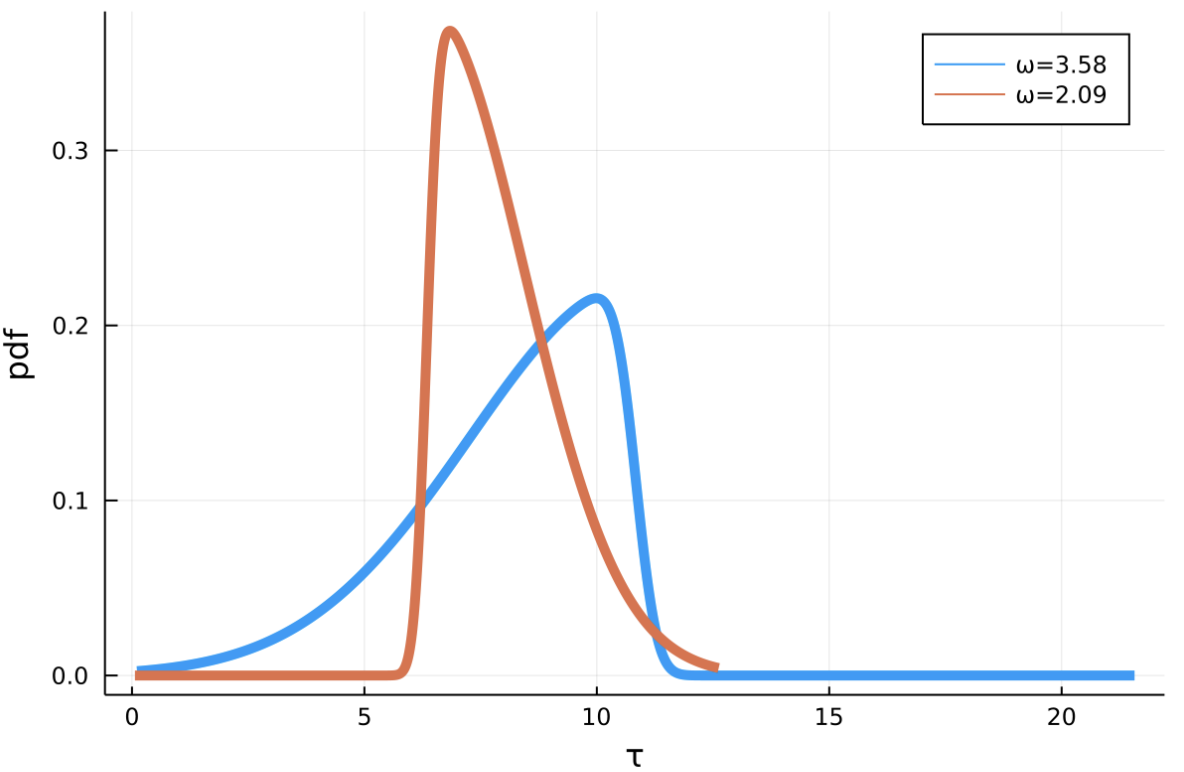
\includegraphics[width=7cm,height=4.75cm]{distskew8.png}
        \caption{pdfs of skewed truncated Gaussian distributions, with $\rho=-10,10$. Both pdfs have mean $\tau=8$.}
        \label{}
    \end{subfigure}
    \hfill
    \begin{subfigure}[t]{0.45\textwidth}
        \centering
        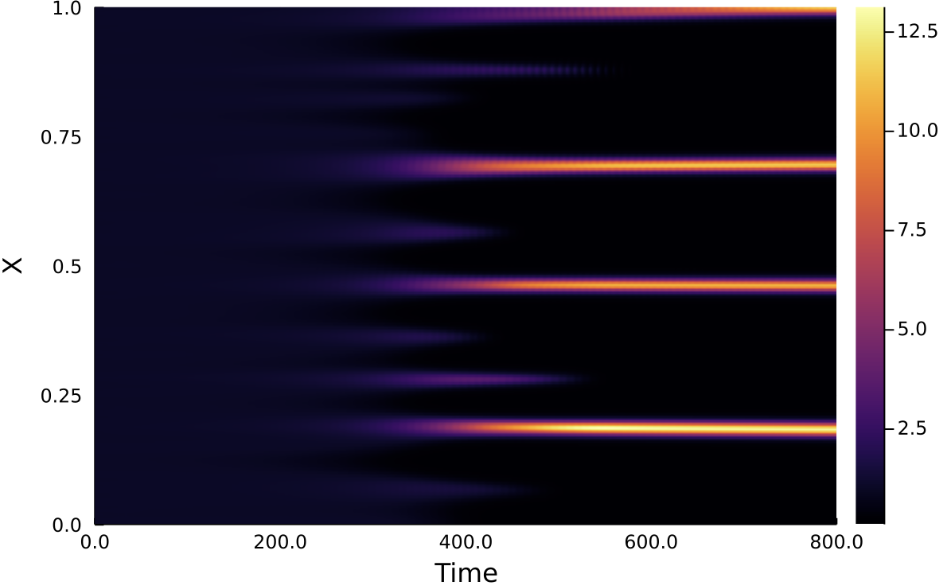
\includegraphics[width=7cm,height=4.75cm]{fixt8.png}
        \caption{Numerical simulation of fixed delay case with $\tau=8$.}
        \label{}
    \end{subfigure}
    \hfill
    \begin{subfigure}[t]{0.45\textwidth}
        \centering
        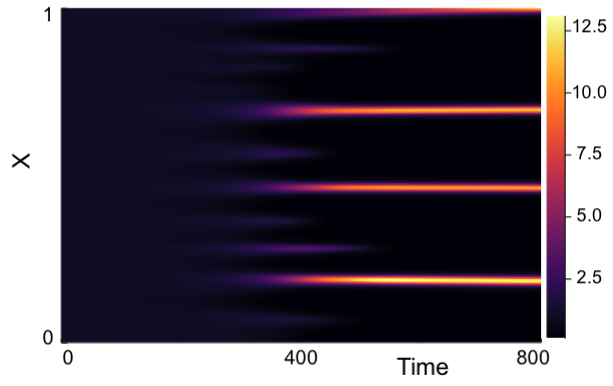
\includegraphics[width=7cm,height=4.75cm]{skewt8m10.png}
        \caption{Numerical simulation with skewed distribution of $\rho=-10$. Distribution parameters are $\mu=10.8(3.s.f)$ and $\omega=3.58(3.s.f)$.}
        \label{}
    \end{subfigure}
    \hfill
    \begin{subfigure}[t]{0.45\textwidth}
        \centering
        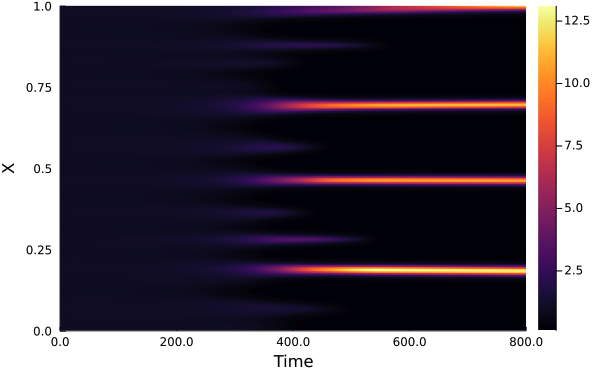
\includegraphics[width=7cm,height=4.75cm]{skewt810.png}
        \caption{Numerical simulation with skewed distribution of $\rho=10$. Distribution parameters are $\mu=6.34(3.s.f)$ and $\omega=2.09(3.s.f)$.}
        \label{}
    \end{subfigure}
    \caption{Numerical rsesults for $(a,b)=(0.1,0.9)$ with $\rho=-10,10$ and $\tau=8$. Parameters $\epsilon^2=0.01$ and $L^2=9/2$. Initial conditions given by \eqref{firstic} and boundary conditions by \eqref{neumannbc}.}
    \label{fig:linskew2}
\end{figure}

\begin{figure}[H]
    \centering
    \begin{subfigure}[t]{0.45\textwidth}
        \centering
        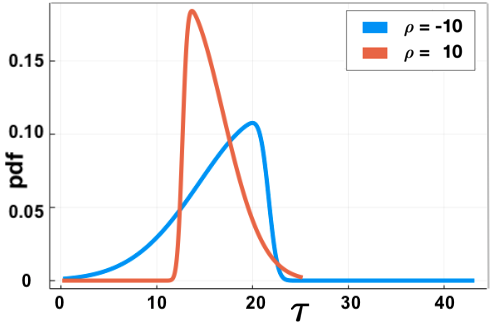
\includegraphics[width=7cm,height=4.75cm]{dist16.png}
        \caption{pdfs of skewed truncated Gaussian distributions, with $\rho=-10,10$. Both pdfs have mean $\tau=16$.}
        \label{}
    \end{subfigure}
    \hfill
    \begin{subfigure}[t]{0.45\textwidth}
        \centering
        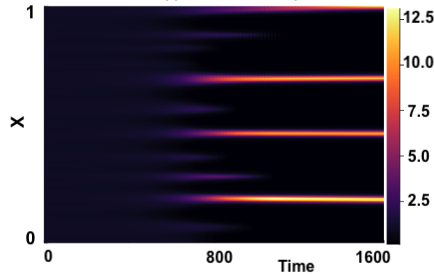
\includegraphics[width=7cm,height=4.75cm]{fixt16.png}
        \caption{Numerical simulation of fixed delay case with $\tau=16$.}
        \label{}
    \end{subfigure}
    \hfill
    \begin{subfigure}[t]{0.45\textwidth}
        \centering
        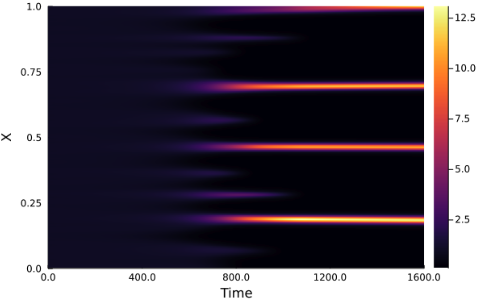
\includegraphics[width=7cm,height=4.75cm]{t16m10.png}
        \caption{Numerical simulation with distribution of $\rho=-10$. Distribution parameters are $\mu=21.7(3.s.f)$ and $\omega=7.16(3.s.f)$.}
        \label{}
    \end{subfigure}
    \hfill
    \begin{subfigure}[t]{0.45\textwidth}
        \centering
        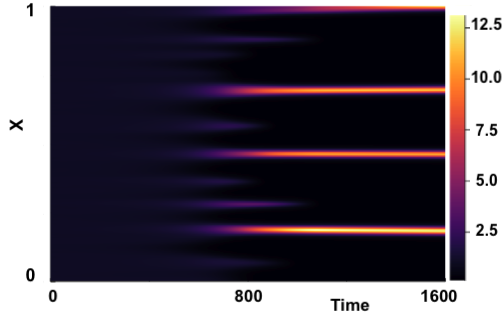
\includegraphics[width=7cm,height=4.75cm]{t1610.png}
        \caption{Numerical simulation with distribution of $\rho=10$. Distribution parameters are $\mu=12.7(3.s.f)$ and $\omega=4.18(3.s.f)$.}
        \label{}
    \end{subfigure}
    \caption{Numerical rsesults for $(a,b)=(0.1,0.9)$ with $\rho=-10,10$ and $\tau=16$. Parameters $\epsilon^2=0.01$ and $L^2=9/2$. Initial conditions given by \eqref{firstic} and boundary conditions by \eqref{neumannbc}.}
    \label{fig:linskew3}
\end{figure}
